% ******************************* PhD Thesis Template **************************
% Please have a look at the README.md file for info on how to use the template

\documentclass[a4paper,12pt,numbered,print,index]{Classes/PhDThesisPSnPDF}

% ******************************************************************************
% ******************************* Class Options ********************************
% *********************** See README for more details **************************
% ******************************************************************************

% `a4paper'(The University of Cambridge PhD thesis guidelines recommends a page
% size a4 - default option) or `a5paper': A5 Paper size is also allowed as per
% the Cambridge University Engineering Deparment guidelines for PhD thesis
%
% `11pt' or `12pt'(default): Font Size 10pt is NOT recommended by the University
% guidelines
%
% `oneside' or `twoside'(default): Printing double side (twoside) or single
% side.
%
% `print': Use `print' for print version with appropriate margins and page
% layout. Leaving the options field blank will activate Online version.
%
% `index': For index at the end of the thesis
%
% `draftclassic': For draft mode without loading any images (same as draft in book)
%
% `draft': Special draft mode with line numbers, images, and water mark with
% timestamp and custom text. Position of the text can also be modified.
%
% `abstract': To generate only the title page and abstract page with
% dissertation title and name, to submit to the Student Registry
%
% `chapter`: This option enables only the specified chapter and it's references
%  Useful for review and corrections.
%
% ************************* Custom Page Margins ********************************
%
% `custommargin`: Use `custommargin' in options to activate custom page margins,
% which can be defined in the preamble.tex. Custom margin will override
% print/online margin setup.
%
% *********************** Choosing the Fonts in Class Options ******************
%
% `times' : Times font with math support. (The Cambridge University guidelines
% recommend using times)
%
% `fourier': Utopia Font with Fourier Math font (Font has to be installed)
%            It's a free font.
%
% `customfont': Use `customfont' option in the document class and load the
% package in the preamble.tex
%
% default or leave empty: `Latin Modern' font will be loaded.
%
% ********************** Choosing the Bibliography style ***********************
%
% `authoryear': For author-year citation eg., Krishna (2013)
%
% `numbered': (Default Option) For numbered and sorted citation e.g., [1,5,2]
%
% `custombib': Define your own bibliography style in the `preamble.tex' file.
%              `\RequirePackage[square, sort, numbers, authoryear]{natbib}'.
%              This can be also used to load biblatex instead of natbib
%              (See Preamble)
%
% **************************** Choosing the Page Style *************************
%
% `default (leave empty)': For Page Numbers in Header (Left Even, Right Odd) and
% Chapter Name in Header (Right Even) and Section Name (Left Odd). Blank Footer.
%
% `PageStyleI': Chapter Name next & Page Number on Even Side (Left Even).
% Section Name & Page Number in Header on Odd Side (Right Odd). Footer is empty.
%
% `PageStyleII': Chapter Name on Even Side (Left Even) in Header. Section Number
% and Section Name in Header on Odd Side (Right Odd). Page numbering in footer

% Uncomment to change page style
%\pagestyle{PageStyleII}

% ********************************** Preamble **********************************
% Preamble: Contains packages and user-defined commands and settings
% ******************************************************************************
% ****************************** Custom Margin *********************************

% Add `custommargin' in the document class options to use this section
% Set {innerside margin / outerside margin / topmargin / bottom margin}  and
% other page dimensions
\ifsetCustomMargin
  \RequirePackage[left=37mm,right=30mm,top=35mm,bottom=30mm]{geometry}
  \setFancyHdr % To apply fancy header after geometry package is loaded
\fi

% Add spaces between paragraphs
%\setlength{\parskip}{0.5em}
% Ragged bottom avoids extra whitespaces between paragraphs
\raggedbottom
% To remove the excess top spacing for enumeration, list and description
%\usepackage{enumitem}
%\setlist[enumerate,itemize,description]{topsep=0em}

% *****************************************************************************
% ******************* Fonts (like different typewriter fonts etc.)*************

% Add `customfont' in the document class option to use this section

\ifsetCustomFont
  % Set your custom font here and use `customfont' in options. Leave empty to
  % load computer modern font (default LaTeX font).
  %\RequirePackage{helvet}

  % For use with XeLaTeX
  %  \setmainfont[
  %    Path              = ./libertine/opentype/,
  %    Extension         = .otf,
  %    UprightFont = LinLibertine_R,
  %    BoldFont = LinLibertine_RZ, % Linux Libertine O Regular Semibold
  %    ItalicFont = LinLibertine_RI,
  %    BoldItalicFont = LinLibertine_RZI, % Linux Libertine O Regular Semibold Italic
  %  ]
  %  {libertine}
  %  % load font from system font
  %  \newfontfamily\libertinesystemfont{Linux Libertine O}
\fi

% *****************************************************************************
% **************************** Custom Packages ********************************

% ************************* Algorithms and Pseudocode **************************

%\usepackage{algpseudocode}


% ********************Captions and Hyperreferencing / URL **********************

% Captions: This makes captions of figures use a boldfaced small font.
%\RequirePackage[small,bf]{caption}

\RequirePackage[labelsep=space,tableposition=top]{caption}
\renewcommand{\figurename}{Fig.} %to support older versions of captions.sty


% *************************** Graphics and figures *****************************

%\usepackage{rotating}
%\usepackage{wrapfig}

% Uncomment the following two lines to force Latex to place the figure.
% Use [H] when including graphics. Note 'H' instead of 'h'
%\usepackage{float}
%\restylefloat{figure}

% Subcaption package is also available in the sty folder you can use that by
% uncommenting the following line
% This is for people stuck with older versions of texlive
%\usepackage{sty/caption/subcaption}
%\usepackage{subcaption}
%\usepackage{graphicx}

% ********************************** Tables ************************************
\usepackage{booktabs} % For professional looking tables
\usepackage{multirow}

%\usepackage{multicol}
%\usepackage{longtable}
%\usepackage{tabularx}


% *********************************** SI Units *********************************
\usepackage{siunitx} % use this package module for SI units


% ******************************* Line Spacing *********************************

% Choose linespacing as appropriate. Default is one-half line spacing as per the
% University guidelines

% \doublespacing
% \onehalfspacing
% \singlespacing


% ************************ Formatting / Footnote *******************************

% Don't break enumeration (etc.) across pages in an ugly manner (default 10000)
%\clubpenalty=500
%\widowpenalty=500

%\usepackage[perpage]{footmisc} %Range of footnote options


% *****************************************************************************
% *************************** Bibliography  and References ********************

%\usepackage{cleveref} %Referencing without need to explicitly state fig /table

% Add `custombib' in the document class option to use this section
\ifuseCustomBib
   \RequirePackage[square, sort, numbers, authoryear]{natbib} % CustomBib

% If you would like to use biblatex for your reference management, as opposed to the default `natbibpackage` pass the option `custombib` in the document class. Comment out the previous line to make sure you don't load the natbib package. Uncomment the following lines and specify the location of references.bib file

%\RequirePackage[backend=biber, style=numeric-comp, citestyle=numeric, sorting=nty, natbib=true]{biblatex}
%\bibliography{References/references} %Location of references.bib only for biblatex

\fi

% changes the default name `Bibliography` -> `References'
\renewcommand{\bibname}{References}


% ******************************************************************************
% ************************* User Defined Commands ******************************
% ******************************************************************************

% *********** To change the name of Table of Contents / LOF and LOT ************

%\renewcommand{\contentsname}{My Table of Contents}
%\renewcommand{\listfigurename}{My List of Figures}
%\renewcommand{\listtablename}{My List of Tables}


% ********************** TOC depth and numbering depth *************************

\setcounter{secnumdepth}{2}
\setcounter{tocdepth}{2}


% ******************************* Nomenclature *********************************

% To change the name of the Nomenclature section, uncomment the following line

%\renewcommand{\nomname}{Symbols}


% ********************************* Appendix ***********************************

% The default value of both \appendixtocname and \appendixpagename is `Appendices'. These names can all be changed via:

%\renewcommand{\appendixtocname}{List of appendices}
%\renewcommand{\appendixname}{Appndx}

% *********************** Configure Draft Mode **********************************

% Uncomment to disable figures in `draft'
%\setkeys{Gin}{draft=true}  % set draft to false to enable figures in `draft'

% These options are active only during the draft mode
% Default text is "Draft"
%\SetDraftText{DRAFT}

% Default Watermark location is top. Location (top/bottom)
%\SetDraftWMPosition{bottom}

% Draft Version - default is v1.0
%\SetDraftVersion{v1.1}

% Draft Text grayscale value (should be between 0-black and 1-white)
% Default value is 0.75
%\SetDraftGrayScale{0.8}


% ******************************** Todo Notes **********************************
%% Uncomment the following lines to have todonotes.

%\ifsetDraft
%	\usepackage[colorinlistoftodos]{todonotes}
%	\newcommand{\mynote}[1]{\todo[author=kks32,size=\small,inline,color=green!40]{#1}}
%\else
%	\newcommand{\mynote}[1]{}
%	\newcommand{\listoftodos}{}
%\fi

% Example todo: \mynote{Hey! I have a note}

\usepackage{graphicx}
\usepackage{subcaption}
\usepackage{amsmath}
\usepackage{algorithm}
\usepackage{amssymb}
\usepackage{amsmath}
\usepackage{amsthm}
\usepackage[noend]{algpseudocode}
\usepackage[utf8]{inputenc}
\usepackage{pgfplots}
\pgfplotsset{width=10cm,compat=1.9}
%\usepackage{texcomp}



% ************************ Thesis Information & Meta-data **********************
% Thesis title and author information, refernce file for biblatex
% ************************ Thesis Information & Meta-data **********************
%% The title of the thesis
\title{SCE17-0037:\\Experimental Analysis of the Application of the gSketch Partitioning Method onto the gMatrix Graph-Stream Sketch}
%\texorpdfstring is used for PDF metadata. Usage:
%\texorpdfstring{LaTeX_Version}{PDF Version (non-latex)} eg.,
%\texorpdfstring{$sigma$}{sigma}

%% Subtitle (Optional)
%\subtitle{Using the CUED template}

%% The full name of the author
\author{Eric Leonardo Lim \\ U1420158D}

%% Department (eg. Department of Engineering, Maths, Physics)
\dept{School of Computer Science and Engineering}

%% University and Crest
\university{Nanyang Technological University}
% Crest minimum should be 30mm.
\crest{
\includegraphics[width=0.75\textwidth]{ntu}}
%% Use this crest, if you are using the college crest
%% Crest long miminum should be 65mm
%\crest{
\includegraphics[width=0.45\textwidth]{University_Crest_Long}}

%% College shield [optional] 
% Crest minimum should be 30mm.
%\collegeshield{
\includegraphics[width=0.2\textwidth]{CollegeShields/Kings}}


%% Supervisor (optional)
%% for multiple supervisors, append each supervisor with the \newline command
\supervisor{Ast/P Arijit Khan}

%% Supervisor Role (optional) - Supervisor (default) or advisor
% \supervisorrole{\textbf{Supervisors: }}
%% if no title is desired:
% \supervisorrole{}

%% Supervisor line width: required to align supervisors
%\supervisorlinewidth{0.35\textwidth}

%% Advisor (optional)
%% for multiple advisors, append each advisor with the \newline command
%\advisor{Dr. A. Advisor\newline
%Dr. B. Advisor}
     
%% Advisor Role (optional) - Advisor (default) or leave empty
% \advisorrole{Advisors: }
%% if no title is required
% \advisorrole{}

%% Advisor line width: required to align supervisors
%\advisorlinewidth{0.25\textwidth}


%% You can redefine the submission text:
% Default as per the University guidelines:
% ``This dissertation is submitted for the degree of''
\renewcommand{\submissiontext}{Submitted in partial fulfilment of the requirements for the degree of}

%% Full title of the Degree
\degreetitle{Bachelor of Engineering (Computer Science)}

%% College affiliation (optional)
%\college{King's College}

%% Submission date
% Default is set as {\monthname[\the\month]\space\the\year}
\degreedate{AY2017/2018} 

%% Meta information
\subject{Partitioning on gMatrix} \keywords{{gMatrix} {Partitioning} {Sketch} {Data Stream} {Graph Stream}}


% ***************************** Abstract Separate ******************************
% To printout only the titlepage and the abstract with the PhD title and the
% author name for submission to the Student Registry, use the `abstract' option in
% the document class.

\ifdefineAbstract
 \pagestyle{empty}
 \includeonly{Declaration/declaration, Abstract/abstract}
\fi

% ***************************** Chapter Mode ***********************************
% The chapter mode allows user to only print particular chapters with references
% Title, Contents, Frontmatter are disabled by default
% Useful option to review a particular chapter or to send it to supervisior.
% To use choose `chapter' option in the document class

\ifdefineChapter
 \includeonly{Chapter3/chapter3}
\fi

\newtheorem{theorem}{Theorem}
\newtheorem*{remarks}{Remarks}
% ******************************** Front Matter ********************************
\begin{document}

\frontmatter

\maketitle

%% ******************************* Thesis Declaration ***************************

\begin{submission}

Fuck you bitch. I hereby declare that except where specific reference is made to the work of 
others, the contents of this dissertation are original and have not been 
submitted in whole or in part for consideration for any other degree or 
qualification in this, or any other university. This dissertation is my own 
work and contains nothing which is the outcome of work done in collaboration 
with others, except as specified in the text and Acknowledgements. This 
dissertation contains fewer than 65,000 words including appendices, 
bibliography, footnotes, tables and equations and has fewer than 150 figures.

% Author and date will be inserted automatically from thesis.tex \author \degreedate

\end{submission}

%% ******************************* Thesis Dedidcation ********************************

\begin{dedication} 

Submitted in Partial Fulfilment of the Requirements for the
Degree of

Bachelor of Engineering (Computer Science) of the

Nanyang Technological University

by Eric Leonardo Lim

\vspace{5mm}

Supervisor: Ast/P Arjit Khan

Examiner: Dr Vivek Chaturvedi

\end{dedication}

%% ******************************* Thesis Declaration ***************************

\begin{declaration}

I hereby declare that except where specific reference is made to the work of 
others, the contents of this dissertation are original and have not been 
submitted in whole or in part for consideration for any other degree or 
qualification in this, or any other university. This dissertation is my own 
work and contains nothing which is the outcome of work done in collaboration 
with others, except as specified in the text and Acknowledgements. This 
dissertation contains fewer than 65,000 words including appendices, 
bibliography, footnotes, tables and equations and has fewer than 150 figures.

% Author and date will be inserted automatically from thesis.tex \author \degreedate

\end{declaration}
% ************************** Thesis Acknowledgements **************************

\begin{acknowledgements}      

I would like to express my gratitude to everyone who gave me the possibility to complete this report. A special thanks to my final year project supervisor, Asst/Prof Arijit Khan, who has provided me with relevant guidance on the project.

\end{acknowledgements}

% ************************** Thesis Abstract *****************************
% Use `abstract' as an option in the document class to print only the titlepage and the abstract.
\begin{abstract}
This report presents a final year project that is about an experimental analysis of applying the gSketch partitioning method onto the gMatrix graph-stream sketch. The report first introduces how the gSketch partitioning method can be applied onto the gMatrix sketch and proposes optimizations for the method, and then analyzes how the gSketch partitioning method changes how gMatrix answers various query types, such as edge frequency, heavy-hitter edges, and node aggregate-frequency queries, and how the performance and probabilistic accuracy guarantees change, and after that, shows experimental results with metrics that each evaluates differently how partitioning affects gMatrix's accuracy for answering the different query types on up to three different graph-stream datasets. Finally, the report concludes that the gSketch partitioning method successfully improves the accuracy of gMatrix in query types such as edge frequency estimation and source-node aggregate-frequency estimation, although fails to bring the same improvements onto the destination-node aggregate-frequency estimation and heavy-hitter edge queries.
\end{abstract}


% *********************** Adding TOC and List of Figures ***********************

\tableofcontents

\listoffigures

%\listoftables

% \printnomenclature[space] space can be set as 2em between symbol and description
%\printnomenclature[3em]

\printnomenclature

% ******************************** Main Matter *********************************
\mainmatter

%!TEX root = ../thesis.tex
%*******************************************************************************
%*********************************** First Chapter *****************************
%*******************************************************************************

\chapter{Introduction}  %Title of the First Chapter

\ifpdf
    \graphicspath{{Chapter1/Figs/Raster/}{Chapter1/Figs/PDF/}{Chapter1/Figs/}}
\else
    \graphicspath{{Chapter1/Figs/Vector/}{Chapter1/Figs/}}
\fi


%********************************** %First Section  **************************************
\section{Background} %Section - 1.1 

Graphs are naturally used to model data that consists of entities and the relationships between them, with entities represented as nodes and the relationships between a pair of entities represented as edges. Common applications include modelling communication networks, social networks, and the Web. In such applications, graph data is often available as a massive input stream of edges, so computing exact properties of the graph is often not computationally feasible. Thus, sketches, which summarize general data streams, are often used to approximate queries with a particular guaranteed accuracy.


%********************************** %Second Section  *************************************
\section{Objectives} %Section - 1.2

The objective of this work is to improve gMatrix's \cite{khan} accuracy using the idea of partitioning given data sample \cite{DBLP}. Experiments are to be carried on multiple dat

%********************************** % Third Section  *************************************
\section{Relevant Literatures}  %Section - 1.3 
\label{section1.3}

Previous work \cite{DBLP} has introduced a way to utilize the Count-min sketch \cite{cormode2005improved}, which is commonly used to approximate the frequency of events in a general data stream, to approximate the frequency of edges in a graph stream. Furthermore, it \cite{DBLP} has introduced the gSketch, which is a partitioning scheme that exploits typical local structural properties within real world graph datasets by building multiple localized Count-min sketches \cite{cormode2005improved} to summarize a graph stream. It has been shown that the partitioning scheme is able to improve overall accuracy when tested on several large graph datasets.

A recent work \cite{khan} has introduced the gMatrix, which is a sketch that generalizes the Count-min sketch for graph streams. The gMatrix has been shown to be able to handle various queries involving the structural properties of the underlying graph, which is an advantage over the Count-min sketch \cite{DBLP}.

Applying a partitioning scheme identical to the gSketch \cite{DBLP} into the gMatrix \cite{khan} may improve its overall accuracy. However, there are no previous works that have shown if it really is the case and the extent of the improvement.

%!TEX root = ../thesis.tex
%*******************************************************************************
%****************************** Second Chapter *********************************
%*******************************************************************************

\chapter{Design and Analysis}

\ifpdf
    \graphicspath{{Chapter2/Figs/Raster/}{Chapter2/Figs/PDF/}{Chapter2/Figs/}}
\else
    \graphicspath{{Chapter2/Figs/Vector/}{Chapter2/Figs/}}
\fi


\section{Preliminaries}

\subsection{CountMin Sketch}

\subsection{gSketch}

\subsection{gMatrix}

\section{Partitioning Scheme}

We implement the idea of partitioning from \cite{DBLP} onto the gMatrix.

A data sample is needed to perform the partitioning. In the experiment, we perform reservoir sampling on the original dataset to obtain the data sample. The size of the data sample is 5\% of the original size of the dataset.

The gMatrix is divided into partitions. Each partition is associated with a set of source vertices. Each source vertex is then only associated with exactly one partition. Edge $(u,v)$ is stored in one of the partitions if and only if $u$ is in the set of source vertices associated with the partition. The idea of the partitioning is to group edges with similar frequencies in the same partition to improve sketch accuracy.

The statistical variances of the frequencies of edges (from the data sample) with common source vertex are computed. We select source vertices which have variances not exceeding a certain threshold (variance of 100 is used in the experiment). An outlier partition is reserved to store frequencies of edges in the dataset whose source vertex is either not found in the data sample or are not suitable for the purpose of the partitioning, i.e. the statistical variance of the frequencies of all edges with the same source vertex in the data sample is exceeding the threshold.

Determining the right outlier partition size is very critical for the effectiveness of the partitioning, even more so than in partitioning the gSketch\cite{DBLP}. We determine the outlier partition size ratio by estimating the outlier ratio from the data sample. We do so by first splitting the data sample into two; the first consists of 90\% of the whole data sample, and the other split consists of the rest; then, after selecting the suitable source vertices from the first split, the ratio of outliers in the second split is computed, which is essentially the ratio of the number of source vertices in the split not found among the previously-selected source vertices, to the size of the split. Then, it is assigned as the outlier partition size ratio.

The partitioning algorithm is no different than in \cite{DBLP}. 

\begin{algorithm}
\caption{Sketch-Partitioning (Data Sample: $D$)}\label{euclid}
\begin{algorithmic}[1]

\State Create a root node $S$ of the partitioning tree as an
active node;
\State $S.sides \gets h$;
\State $S.depth \gets d$;
\State Create an empty list $L$ containing $S$ only;
\While{$L \neq \varnothing$ }
\State Partition active node $S \in L$ based on D into $S_1$, $S_2$ by minimizing overall relative error;
\State $S_1.rows = S_2.rows = \frac{S.rows}{2};$
\State $L \gets L \setminus \left \{ S \right \};$
\For{$i \in \left[ 1..2 \right]$}
    \If{$(S_i.sides >= w_0)$ and ($\sum_{v \in V_S} \tilde{d}(v) \leqslant C \cdot S_i.sides$)}
    
    \State $L \gets L \cup S_i$;
    \Else
    \State Construct the localized sketch $S_i$;
    
    \EndIf
\EndFor
\EndWhile

\end{algorithmic}
\end{algorithm}

The suitable source vertices are sorted based on non-decreasing average frequency of edges emanating from them $f_v/d_v$ in the data sample, where $f_v$ is the sum of frequencies of all edges in the data sample with source vertex $v$, and $d_v$ is the out-degree of vertex $v$. The sorted source vertex set is then recursively split into two, and each split minimizes the overall relative error E. \[E = \sum_{v \in S_1} \frac{d_v \cdot F_{S_1}}{f_v / d_v} + \sum_{v \in S_2} \frac{d_v \cdot F_{S_1}}{f_v / d_v}\]

The recursion stops when either the size of the partition becomes small enough, i.e. the number of rows is less than a user-specified threshold $r_0$ (which is fixed at 100 in this experiment), or when the probability of collision in any particular cell in the sketch can be bounded above by a user-speficied threshold $C$, which is the case when the density of distinct edges, $\sum_{v \in s} d_v/(S.rows \cdot S.cols)$, is also bounded above by $C$, as proven in \cite{DBLP}.


\section{Edge Frequency Queries}

\subsubsection{Description}
Since there is only one partition associated with each source vertex, to retrieve the estimated frequency for an arbitrary edge $(i,j)$:

\begin{enumerate}
  \item Find partition $p$ that is responsible for $i$
  \item Find the minimum of $V_P(g_k(i),g_k(j),k)$ for all $k \in \{1..w\}$, where $V_P$ is the value of the cell in the partition $p$. 
\end{enumerate}

\subsubsection{Analysis}

Since obtaining the frequency estimate of an arbitrary edge only depends on the partition containing the edge, we observe how each partition answers the query.

Let $S$ be a gMatrix of size $h\times h\times w$. Suppose the partitioning step is performed already. Note that any of the produced partitions will have number of rows equal to $\frac{h}{2^d}$ where $d$ is the depth of the recursion in which the partition is built. Let $p$ be an arbitrary partition. The size of $p$ is $\frac{h}{2^d}\times h\times w$.

\begin{theorem}
\label{efreqguarantee}
Let $(i,j)$ be an edge in $p$, $Q(i,j)$ be its actual frequency, and $\overline{Q(i,j)}$ be its estimated frequency according to partition $p$. Let $L_p$ be the total frequency of edges received so far in the arbitrary partition, i.e. total frequency of edges $(u,v)$ such that $u$ is associated with $p$. Let $A_p(j)$ be the sum of the frequencies of edges $(u,v)$ on $p$ such that $v=j$. Let $B_p(i)$ be the sum of the frequencies of edges $(u,v)$ on $p$ such that $u=i$. Let $\epsilon \in (0,1)$ be a very small fraction. Then,
  
  \[
P(Q(i,j) \leq \overline{Q(i,j)} \leq Q(i,j) + L_p \cdot \epsilon + A_p(j) \cdot h \cdot \epsilon + B_p(i) \cdot h \cdot \epsilon) \geq 1-(\frac{2^{d+1}+1}{h^2\cdot\epsilon})^w
\]

\end{theorem}

\begin{proof}
  Note that $\overline{Q(i,j)}$ is essentially $Q(i,j)$ added with the frequencies of spurious edges mapped into the same cell $(g_k(i),g_k(j),k)$ in the partition, so $P(Q(i,j) \leq \overline{Q(i,j)}) = 1$. We remain to show that

\[
P(\overline{Q(i,j)} \leq Q(i,j) + L_p \cdot \epsilon + A_p(j) \cdot h \cdot \epsilon + B_p(i) \cdot h \cdot \epsilon) \geq 1-(\frac{2^{d+1}+1}{h^2\cdot\epsilon})^w
\]

  There are three possible cases for the spurious edges.
  
The first possible case of spurious edges $(u,v)$ are those for which $u \neq i$ and $v \neq j$. Any of such edges are equally likely to be mapped into any cell in $p$, and the probability to be mapped into any particular cell is $\frac{1}{h \cdot \frac{h}{2^d}} = \frac{2^d}{h^2}$. Let $X_k$ be a random variable that represents the number of such spurious edges that are mapped into $(g_k(i),g_k(j),k)$. Therefore, $E[X_k] = \frac{2^dL_p}{h^2}$. Then, by Markov's inequality,

\begin{equation} \label{efreq1}
P(X_k \geq L_p \cdot \epsilon) \leq \frac{E[X_k]}{L_p \cdot \epsilon} = \frac{2^d}{h^2\epsilon}
\end{equation}

The second possible case of spurious edges $(u,v)$ are those for which $u \neq i$ but $v=j$. The probability that any of such edges to be mapped into $(g_k(i),g_k(j),k)$ in $p$ is $\frac{1}{\frac{h}{2^d}} = \frac{2^d}{h}$. Let $Y_k$ be a random variable representing the number of such spurious edges. Therefore, $E[Y_k] = \frac{2^dA_p(j)}{h}$. By Markov's inequality,

\begin{equation} \label{efreq2}
P(Y_k \geq h A_p(j) \cdot \epsilon) \leq \frac{E[Y_k]}{h A_p(j) \cdot \epsilon} = \frac{2^d}{h^2\epsilon}
\end{equation}

The third possible case of spurious edges $(u,v)$ are those for which $u=i$ but $v \neq j$. The probability that any of such edges to be mapped into $(g_k(i),g_k(j),k)$ in $p$ is $\frac{1}{h}$. Let $Z_k$ be a random variable representing the number of such spurious edges. Therefore, $E[Z_k] = \frac{B_p(i)}{h}$. By Markov's inequality,

\begin{equation} \label{efreq3}
P(Z_k \geq h B_p(i) \cdot \epsilon) \leq \frac{E[Z_k]}{h B_p(i) \cdot \epsilon} = \frac{1}{h^2\epsilon}
\end{equation}

Combining inequations \ref{efreq1}, \ref{efreq2}, \ref{efreq3},
\begin{equation} \label{efreq4}
  P(X_k + Y_k + Z_k \geq L_p \cdot \epsilon + A_p(j) \cdot h \cdot \epsilon + B_p(i) \cdot h \cdot \epsilon) \leq \frac{2^{d+1}+1}{h^2\cdot\epsilon}
\end{equation}

Therefore,
\begin{align}
\begin{split}
&  P(\overline{Q(i,j)} \leq Q(i,j) + L_p \cdot \epsilon + A_p(i) \cdot h \cdot \epsilon + B_p(i) \cdot h \cdot \epsilon)
\\  &= 1 - \prod _{k=1}^{w}P(X_k + Y_k + Z_k \geq L_p \cdot \epsilon + A_p(j) \cdot h \cdot \epsilon + B_p(i) \cdot h \cdot \epsilon)
\\  &\geq 1-(\frac{2^{d+1}+1}{h^2\cdot\epsilon})^w
\end{split}
\end{align}

\end{proof}

\begin{remarks}
  The probability of the guarantee gets lower as the depth $d$ of the recursion in which a partition is built gets deeper, but in ideal partitioning, the guarantee of the estimate of the partition itself gets better as $L_p$, $A_p(i)$, and $B_p(i)$ are reduced.
\end{remarks}


\section{Heavy-hitter Edge Queries}
\subsubsection{Description}
Obtaining edges with frequencies at least $F$ in the graph stream is accomplished by first obtaining a set of edges with frequencies at least $F$ from each partition in the gMatrix and then taking the union of each of them.

\subsubsection{Analysis}

\begin{theorem}
Let $(i,j)$ be an edge and $p$ be the partition associated with $i$. Let $Q(i,j)$ be its actual frequency, and $\overline{Q(i,j)}$ be its estimated frequency according to partition $p$. Let $L_p$ be the total frequency of edges received so far in the arbitrary partition, i.e. total frequency of edges $(u,v)$ such that $u$ is associated with $p$. Let $A_p(j)$ be the sum of the frequencies of edges $(u,v)$ on $p$ such that $v=j$. Let $B_p(i)$ be the sum of the frequencies of edges $(u,v)$ on $p$ such that $u=i$. Let $\epsilon \in (0,1)$ be a very small fraction. Then,
\[
P(Q(i,j) \geq F) \geq 1-(\frac{3\cdot2^d(L_p+h\cdot A_p(j)) + 3\cdot h\cdot B_p(i)}{h^2\cdot (\overline{Q(i,j)}-F)})^w
\]
\end{theorem}

\begin{proof}
Note that if the number of spurious edges is at most $(\overline{Q(i,j)} - F)$, the true frequency $Q(i,j)$ is at least $F$, so by obtaining a lower bound for the probability of the former, we obtain a lower bound for the probability of the latter as well.

To obtain a lower bound for the probability that the number of spurious edges is at most $(\overline{Q(i,j)} - F)$, we consider all possible cases of spurious edges.

The first possible case of spurious edges $(u,v)$ are those for which $u \neq i$ and $v \neq j$. Any of such edges are equally likely to be mapped into any cell in $p$, and the probability to be mapped into any particular cell is $\frac{1}{h \cdot \frac{h}{2^d}} = \frac{2^d}{h^2}$. Let $X_k$ be a random variable that represents the number of such spurious edges that are mapped into $(g_k(i),g_k(j),k)$. Therefore, $E[X_k] = \frac{2^dL_p}{h^2}$. Then, by Markov's inequality,

\begin{equation} \label{hh1}
P(X_k \geq \frac{\overline{Q(i,j)}-F}{3}) \leq \frac{E[X_k]}{\frac{\overline{Q(i,j)}-F}{3}} = \frac{3\cdot2^dL_p}{h^2(\overline{Q(i,j)}-F)}
\end{equation}

The second possible case of spurious edges $(u,v)$ are those for which $u \neq i$ but $v=j$. The probability that any of such edges to be mapped into $(g_k(i),g_k(j),k)$ in $p$ is $\frac{1}{\frac{h}{2^d}} = \frac{2^d}{h}$. Let $Y_k$ be a random variable representing the number of such spurious edges. Therefore, $E[Y_k] = \frac{2^dA_p(j)}{h}$. By Markov's inequality,

\begin{equation} \label{hh2}
P(Y_k \geq \frac{\overline{Q(i,j)}-F}{3}) \leq \frac{E[Y_k]}{\frac{\overline{Q(i,j)}-F}{3}} = \frac{3\cdot2^dA_p(j)}{h(\overline{Q(i,j)}-F)}
\end{equation}

The third possible case of spurious edges $(u,v)$ are those for which $u=i$ but $v \neq j$. The probability that any of such edges to be mapped into $(g_k(i),g_k(j),k)$ in $p$ is $\frac{1}{h}$. Let $Z_k$ be a random variable representing the number of such spurious edges. Therefore, $E[Z_k] = \frac{B_p(i)}{h}$. By Markov's inequality,

\begin{equation} \label{hh3}
P(Z_k \geq \frac{\overline{Q(i,j)}-F}{3}) \leq \frac{E[Z_k]}{\frac{\overline{Q(i,j)}-F}{3}} = \frac{3\cdot B_p(i)}{h(\overline{Q(i,j)}-F)}
\end{equation}

Combining inequations \ref{hh1}, \ref{hh2}, \ref{hh3},
\begin{equation}
  P(X_k + Y_k + Z_k \geq \overline{Q(i,j)}-F) \leq \frac{3\cdot2^d(L_p+h\cdot A_p(j)) + 3\cdot h\cdot B_p(i)}{h^2\cdot (\overline{Q(i,j)}-F)}
\end{equation}

Therefore,
\begin{align}
\begin{split}
&  P(Q(i,j) \geq F)
\\  &= 1 - \prod _{k=1}^{w}P(X_k + Y_k + Z_k \geq \overline{Q(i,j)}-F)
\\  &\geq 1-(\frac{3\cdot2^d(L_p+h\cdot A_p(j)) + 3\cdot h\cdot B_p(i)}{h^2\cdot (\overline{Q(i,j)}-F)})^w
\end{split}
\end{align}

\end{proof}

\section{Node Aggregate-Frequency Queries}

The queries ask for the sum of frequencies of all edges incoming to / outgoing from a node $i$. Due to partitioning based on source nodes, source-node aggregate-frequency queries and destination-node aggregate-frequency queries are computed differently.

\subsection{Source-Node Aggregate-Frequency Queries}

\subsubsection{Description}
The task of finding the aggregate frequency of a source node $i$ is broken down to:

\begin{enumerate}
\item Finding the associated partition $p$ of $i$
\item Finding the aggregate frequency of the source node $i$ at the partition $p$
\end{enumerate}

\subsubsection{Analysis}

\begin{theorem}
Let $(i,j)$ be an edge and $p$ be the partition associated with $i$. Let $Q_{agg}^{+}(i)$ be the true aggregate-frequency of source-node $i$, and $\overline{Q_{agg}^{+}(i)}$ be its estimated aggregate-frequency. Let $p$ be a partition associated with $i$ and $L_p$ be the total frequency of edges received so far on $p$. Let $\epsilon \in (0,1)$ be a very small fraction. Then,
\[
P(Q_{agg}^{+}(i) \leq \overline{Q_{agg}^{+}(i)} \leq Q_{agg}^{+}(i) + L_p \cdot \epsilon) \geq 1-(\frac{2^d}{h\cdot\epsilon})^w
\]
\end{theorem}

\begin{proof}
We note that $P(Q_{agg}^{+}(i) \leq \overline{Q_{agg}^{+}(i)}) = 1$ since $\overline{Q_{agg}^{+}(i)}$ is always an overestimate. We remain to show that
\[
P(\overline{Q_{agg}^{+}(i)} \leq Q_{agg}^{+}(i) + L_p \cdot \epsilon) \geq 1-(\frac{2^d}{h\cdot\epsilon})^w
\]
In any arbitrary partition $p$, the probability for a spurious edge $(u,v)$, where $u \neq i$ and $u$ is associated with $p$, to be mapped onto $(g_k(i),\cdot,k)$ is $\frac{1}{\frac{h}{2^d}} = \frac{2^d}{h}$, so the expected number of spurious edges that are mapped into $(g_k(i),\cdot,k)$ is $\frac{2^dL_p}{h}$. Let $R_k$ be the random variable that represents the number of such spurious edges for the $k^{th}$ hash function. By Markov's inequality,

\begin{equation} \label{agg21}
  P(R_k \geq L_p \epsilon) \leq \frac{E[R_k]}{L_p \epsilon} = \frac{2^d}{h\epsilon}
\end{equation}

Therefore,
\begin{align}
\begin{split}
&  P(\overline{Q_{agg}^{+}(i)} \leq Q_{agg}^{+}(i) + L_p \cdot \epsilon)
\\  &= 1 - \prod _{k=1}^{w}P(R_k \geq L_p \cdot \epsilon)
\\  &\geq 1-(\frac{2^d}{h\cdot\epsilon})^w
\end{split}
\end{align}

\end{proof}

\begin{remarks}
As the depth $d$ of the recursion in which the partition is built increases, the probability of the accuracy guarantee decreases, but in ideal partitioning, the accuracy guarantee itself gets better as $L_p$ gets reduced.
\end{remarks}

\subsection{Destination-Node Aggregate-Frequency Queries}

\subsubsection{Description}
The task of finding the aggregate-frequency of a destination node $j$ is broken down to:

\begin{enumerate}
\item Computing the aggregate-frequency of the destination-node $j$ in each partition $p$
\item Computing the sum of all of the computed destination-node aggregate-frequencies together
\end{enumerate}

\subsubsection{Analysis}
\begin{theorem}
\label{agg2}
  Let $Q_{agg}^{-}(j)$ be the true aggregate-frequency of destination-node $j$, and $\overline{Q_{agg}^{-}(j)}$ be the estimated aggregate-frequency. Let $L$ be the total frequency of edges received so far. Let $\epsilon \in (0,1)$ be a very small fraction. Then,
  
  \[
P(Q_{agg}^{-}(j) \leq \overline{Q_{agg}^{-}(j)} \leq Q_{agg}^{-}(j) + L \cdot \epsilon) \geq 1-(\frac{n}{h\cdot\epsilon})^w
\]

\end{theorem}

\begin{proof}
We note that $P(Q_{agg}^{-}(j) \leq \overline{Q_{agg}^{-}(j)}) = 1$ since $\overline{Q_{agg}^{-}(j)}$ is always an overestimate. We remain to show that
\[
P(\overline{Q_{agg}^{-}(j)} \leq Q_{agg}^{-}(j) + L \cdot \epsilon) \geq 1-(\frac{n}{h\cdot\epsilon})^w
\]
Let $\{p_1,..,p_n\}$ be the set of all partitions in the gMatrix and $L_i$ be the total frequency of edges in $p_i$. In any partition $p_i$, the probability for a spurious edge $(u,v)$, $v \neq j$ to be mapped onto $(\cdot,g_k(j),k)$ is $\frac{1}{h}$, so the expected number of spurious edges that are mapped into $(\cdot,g_k(j),k)$ is $\frac{L_i}{h}$. Let $R_k^i$ be the random variable that represents the number of spurious edges in $p_i$ for the $k^{th}$ hash function. By Markov's inequality,

\begin{equation} \label{agg21}
  P(R_k^i \geq L_i \epsilon) \leq \frac{E[R_k^i]}{L_i \epsilon} = \frac{1}{h\epsilon}
\end{equation}

Let $R_k = \sum_{i=1}^{n} R_k^i$. Combining inequation \ref{agg21} for all $i \in \{1..n\}$, 

\begin{equation} \label{agg22}
 P(R_k \geq L\epsilon) \leq \frac{n}{h\epsilon}
\end{equation}

Therefore,
\begin{align}
\begin{split}
&  P(\overline{Q_{agg}^{-}(j)} \leq Q_{agg}^{-}(j) + L \cdot \epsilon)
\\  &= 1 - \prod _{k=1}^{w}P(R_k \geq L \cdot \epsilon)
\\  &\geq 1-(\frac{n}{h\cdot\epsilon})^w
\end{split}
\end{align}

\end{proof}

\begin{remarks}
The probability of the guarantee gets lower as the number of partitions increases, and the guarantee itself never gets any better with partitioning.
\end{remarks}

%!TEX root = ../thesis.tex
%*******************************************************************************
%****************************** Third Chapter **********************************
%*******************************************************************************
\chapter{Experiments}

% **************************** Define Graphics Path **************************
\ifpdf
    \graphicspath{{Chapter3/Figs/Raster/}{Chapter3/Figs/PDF/}{Chapter3/Figs/}}
\else
    \graphicspath{{Chapter3/Figs/Vector/}{Chapter3/Figs/}}
\fi

We compare the accuracy of gMatrix without partitioning and with partitioning for answering edge frequency estimation queries.

\section{Implementation}
In this experiment, the data sample needed for partitioning is obtained by performing reservoir sampling\cite{DBLP} on the graph stream. Each data sample consists of 5\% random edges from the graph stream.

Statistical threshold of 100 is used to filter source nodes of the data sample.

For outlier ratio estimation, data sample is split by 90:10 ratio.

\section{System Description}
The code is implemented in C++ and experiments were performed on Intel Xeon 2GHz 16GB server.

\section{Datasets}
The datasets used to evaluate the sketches are graph streams consisting of distinct edges only. The datasets are:
\begin{itemize}
\item IP-Trace Network Stream \cite{khan}
\item Twitter Communication Stream \cite{khan}
\item Friendster Stream with Zipf Frequency distribution \cite{khan}
\end{itemize}

\section{Metrics}
\subsection{Edge Frequency \& Node Aggregate-Frequency Estimation}
\subsubsection{Observed Error \cite{khan}}
\[
observed\;error = \frac{ \sum_{i=1}^{|Q|}{|\tilde{f}(q_i) - f(q_i)|} }{\sum_{i=1}^{|Q|}f(q_i)}
\]
where $Q = \{q_i\}$ is the set of queries, $\tilde{f}$ is the estimated frequency, and $f$ is the actual frequency.

\subsubsection{Average Relative Error \cite{DBLP}}
\[
average\;relative\;error = \frac{1}{|Q|} \sum_{i=1}^{|Q|} \frac{\tilde{f}(q_i)-f(q_i)}{f(q_i)}
\]
where $Q = \{q_i\}$ is the set of queries, $\tilde{f}$ is the estimated frequency, and $f$ is the actual frequency.

\subsubsection{Effective Queries \cite{DBLP}}
Both Observed Error and Average Relative Error may be biased if the frequencies of the queries vary a lot, so we define queries as "effective" if the relative error is not exceeding $T$. The percentage of effective queries is computed by,
\[
effective\;queries = \frac{|\{q|\frac{\tilde{f}(q)-f(q)}{f(q)} \leq T, q \in Q\}|}{|Q|} \cdot 100\%
\]
where $Q = \{q_i\}$ is the set of queries, $\tilde{f}$ is the estimated frequency, and $f$ is the actual frequency.

In this experiment, $T$ is set to 5, which is the same as \cite{DBLP}.

\subsection{Heavy Hitter Edge Estimation}
\subsubsection{False Positive Rate \cite{khan}}

\[
false\;positive\;rate(\%) = \frac{#false\;heavyhitter\;edges}{#true\;heavyhitter\;edges} \cdot 100\%
\]

\clearpage
\section{Results}

\subsection{Edge Frequency Estimation}

\paragraph{Friendster dataset}
Partitioning reduces the observed error and the average relative error of the estimations, as seen on figures \ref{fig:F11}-\ref{fig:F21}. The lower errors are possible because partitioning reduces the number of queries with high relative errors (queries $q$ such that $\frac{\tilde{f}(q)-f(q)}{f(q)} > T$), as the number of effective queries themselves are actually lower with partitioning as seen on figure \ref{fig:F31}.

\paragraph{Twitter dataset}
Partitioning does not seem to be effective at all as seen on figures \ref{fig:T11}-\ref{fig:T32}.

\paragraph{IP-Trace dataset}
Partitioning reduces the observed error and the average relative error of the estimations, as seen on figures \ref{fig:I11}-\ref{fig:I21}. Unlike the results on the Friendster dataset, the number of effective queries after partitioning are only significantly lower on $h=1000$ and is actually higher than without partitioning on $h=4000$.

%Friendster
%Observed error

\begin{figure}[!htbp]
\centering
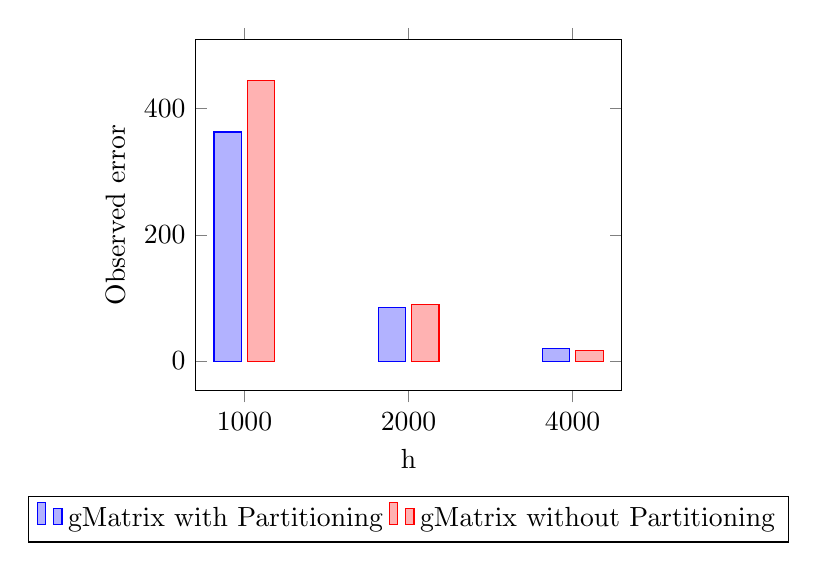
\begin{tikzpicture}
  \begin{axis}[
      ybar,
      enlargelimits=0.15,
      legend style={at={(0.5,-0.3)},anchor=north,legend columns=-1},
      ylabel={Observed error},
      xlabel={h},
      width=7cm,
      symbolic x coords={1000,2000,4000},
      xtick=data
    ]
      \addplot 
	  coordinates {
        (1000,  362.84)
        (2000,  85.24)
        (4000,  19.31)
      };
      \addplot 
	  coordinates {
        (1000,  444.81)
        (2000,  90.16)
        (4000,  17.30)
      };
      \legend{gMatrix with Partitioning,gMatrix without Partitioning}
  \end{axis}
\end{tikzpicture}
\caption{Observed error on Friendster dataset considered over 1 million random edges} \label{fig:F11}
\end{figure}

\begin{figure}[!htbp]
\centering
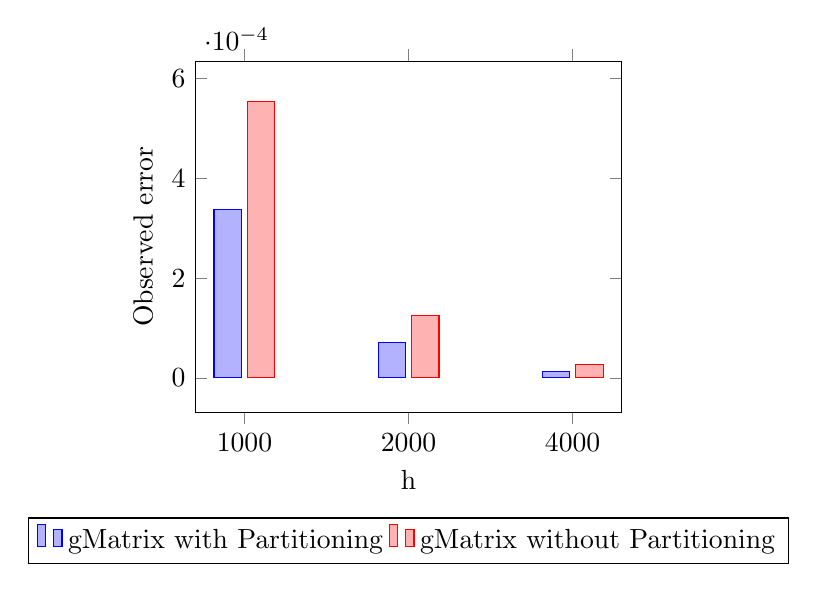
\begin{tikzpicture}
  \begin{axis}[
      ybar,
      enlargelimits=0.15,
      legend style={at={(0.5,-0.3)},anchor=north,legend columns=-1},
      ylabel={Observed error},
      xlabel={h},
      width=7cm,
      symbolic x coords={1000,2000,4000},
      xtick=data
    ]
      \addplot 
	  coordinates {
        (1000,  0.000338304)
        (2000,  7.17931e-05)
        (4000,  1.25923e-05)
      };
      \addplot 
	  coordinates {
        (1000,  0.000553365)
        (2000,  0.000124219)
        (4000,  2.61629e-05)
      };
      \legend{gMatrix with Partitioning, gMatrix without Partitioning}
  \end{axis}
\end{tikzpicture}
\caption{Observed error on Friendster dataset considered over top-500 highest frequency edges} \label{fig:F12}
\end{figure}

% Average relative error

\begin{figure}[!htbp]
\centering
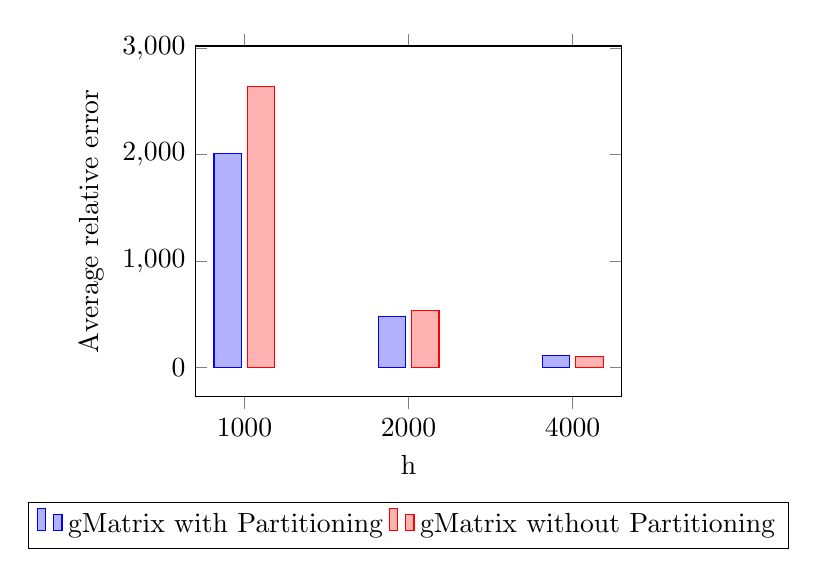
\begin{tikzpicture}
  \begin{axis}[
      ybar,
      enlargelimits=0.15,
      legend style={at={(0.5,-0.3)},anchor=north,legend columns=-1},
      ylabel={Average relative error},
      xlabel={h},
      width=7cm,
      symbolic x coords={1000,2000,4000},
      xtick=data
    ]
      \addplot 
	  coordinates {
        (1000,  2009.98)
        (2000,  478.512)
        (4000,  110.623)
      };
      \addplot 
	  coordinates {
        (1000,  2642.89)
        (2000,  535.386)
        (4000,  102.601)
      };
      \legend{gMatrix with Partitioning,gMatrix without Partitioning}
  \end{axis}
\end{tikzpicture}
\caption{Average relative error on Friendster dataset considered over 1 million random edges} \label{fig:F21}
\end{figure}

\begin{figure}[!htbp]
\centering
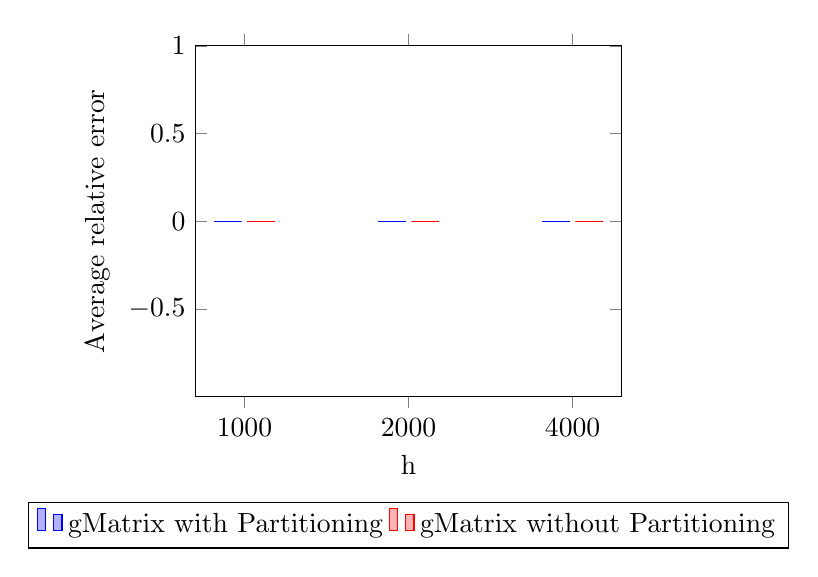
\begin{tikzpicture}
  \begin{axis}[
      ybar,
      enlargelimits=0.15,
      legend style={at={(0.5,-0.3)},anchor=north,legend columns=-1},
      ylabel={Average relative error},
      xlabel={h},
      width=7cm,
      symbolic x coords={1000,2000,4000},
      xtick=data
    ]
      \addplot 
	  coordinates {
        (1000,  0)
        (2000,  0)
        (4000,  0)
      };
      \addplot 
	  coordinates {
        (1000,  0)
        (2000,  0)
        (4000,  0)
      };
      \legend{gMatrix with Partitioning, gMatrix without Partitioning}
  \end{axis}
\end{tikzpicture}
\caption{Average relative error on Friendster dataset considered over top-500 highest frequency edges} \label{fig:F22}
\end{figure}

% Effective queries

\begin{figure}[!htbp]
\centering
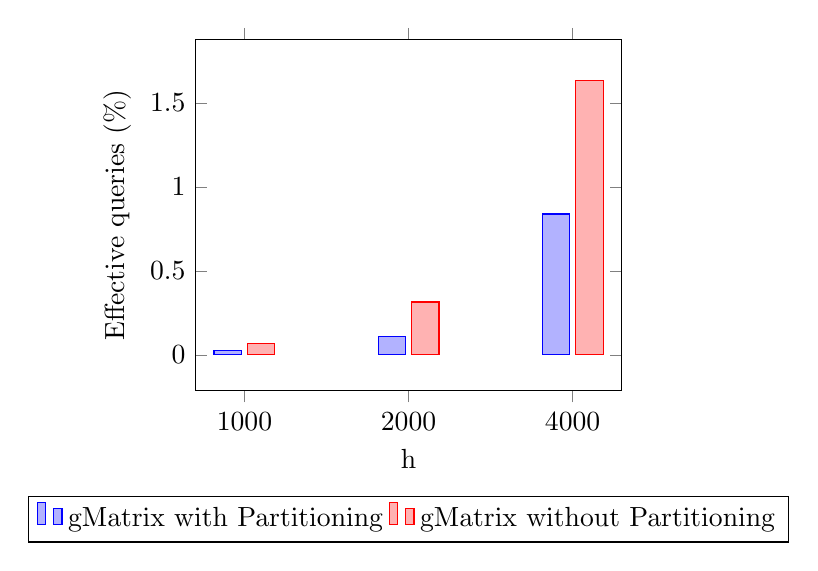
\begin{tikzpicture}
  \begin{axis}[
      ybar,
      enlargelimits=0.15,
      legend style={at={(0.5,-0.3)},anchor=north,legend columns=-1},
      ylabel={Effective queries (\%)},
      xlabel={h},
      width=7cm,
      symbolic x coords={1000,2000,4000},
      xtick=data
    ]
      \addplot 
	  coordinates {
        (1000,  0.0285)
        (2000,  0.1098)
        (4000,  0.8383)
      };
      \addplot 
	  coordinates {
        (1000,  0.0671)
        (2000,  0.3152)
        (4000,  1.6345)
      };
      \legend{gMatrix with Partitioning,gMatrix without Partitioning}
  \end{axis}
\end{tikzpicture}
\caption{Effective queries percentage on Friendster dataset considered over 1 million random edges} \label{fig:F31}
\end{figure}

\begin{figure}[!htbp]
\centering
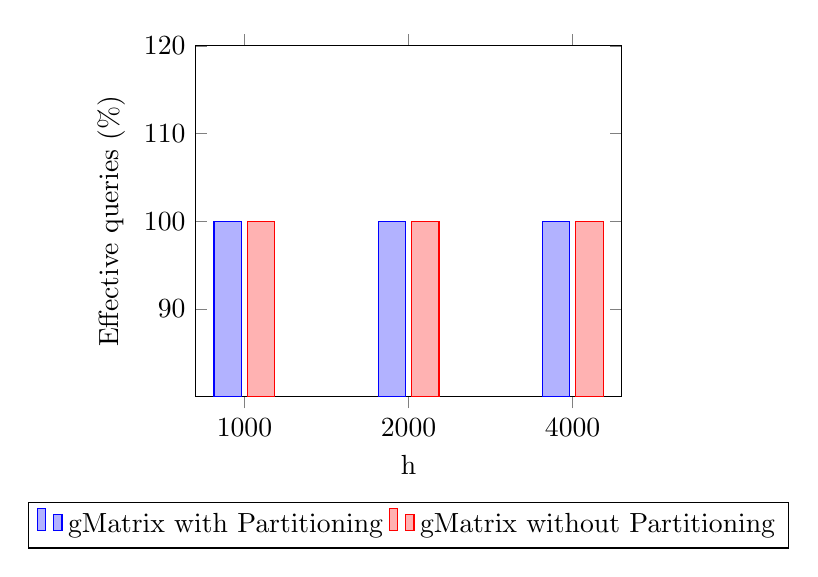
\begin{tikzpicture}
  \begin{axis}[
      ybar,
      enlargelimits=0.15,
      legend style={at={(0.5,-0.3)},anchor=north,legend columns=-1},
      ylabel={Effective queries (\%)},
      xlabel={h},
      width=7cm,
      symbolic x coords={1000,2000,4000},
      xtick=data
    ]
      \addplot 
	  coordinates {
        (1000,  100)
        (2000,  100)
        (4000,  100)
      };
      \addplot 
	  coordinates {
        (1000,  100)
        (2000,  100)
        (4000,  100)
      };
      \legend{gMatrix with Partitioning, gMatrix without Partitioning}
  \end{axis}
\end{tikzpicture}
\caption{Effective queries percentage on Friendster dataset considered over top-500 highest frequency edges} \label{fig:F32}
\end{figure}

%Twitter
%Observed error

\begin{figure}[!htbp]
\centering
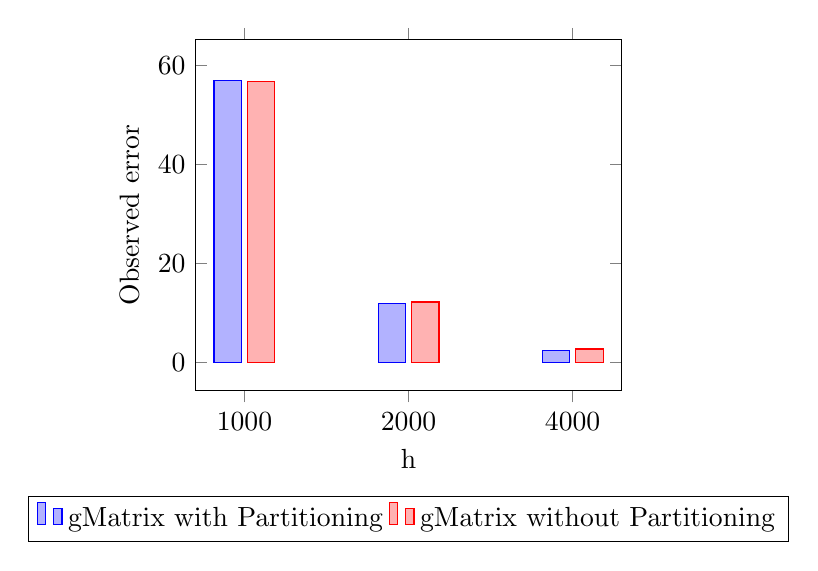
\begin{tikzpicture}
  \begin{axis}[
      ybar,
      enlargelimits=0.15,
      legend style={at={(0.5,-0.3)},anchor=north,legend columns=-1},
      ylabel={Observed error},
      xlabel={h},
      width=7cm,
      symbolic x coords={1000,2000,4000},
      xtick=data
    ]
      \addplot 
	  coordinates {
        (1000,  56.9662)
        (2000,  11.94)
        (4000,  2.4375)
      };
      \addplot 
	  coordinates {
        (1000,  56.7384)
        (2000,  12.1534)
        (4000,  2.67581)
      };
      \legend{gMatrix with Partitioning,gMatrix without Partitioning}
  \end{axis}
\end{tikzpicture}
\caption{Observed error of Twitter dataset considered over 1 million random edges} \label{fig:T11}
\end{figure}

\begin{figure}[!htbp]
\centering
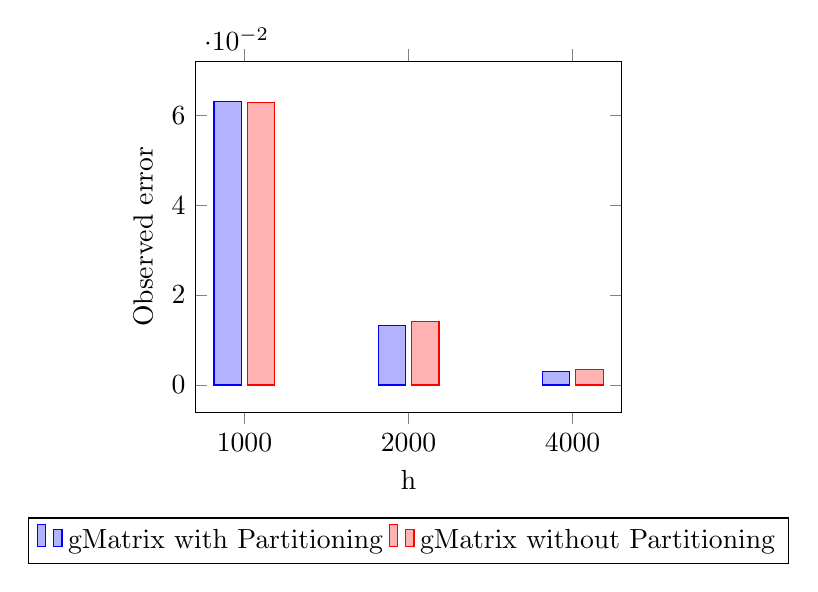
\begin{tikzpicture}
  \begin{axis}[
      ybar,
      enlargelimits=0.15,
      legend style={at={(0.5,-0.3)},anchor=north,legend columns=-1},
      ylabel={Observed error},
      xlabel={h},
      width=7cm,
      symbolic x coords={1000,2000,4000},
      xtick=data
    ]
      \addplot 
	  coordinates {
        (1000,  0.0630049)
        (2000,  0.0132349)
        (4000,  0.00296191)
      };
      \addplot 
	  coordinates {
        (1000,  0.0628949)
        (2000,  0.0140856)
        (4000,  0.00347708)
      };
      \legend{gMatrix with Partitioning, gMatrix without Partitioning}
  \end{axis}
\end{tikzpicture}
\caption{Observed error of Twitter dataset considered over top-500 highest frequency edges} \label{fig:T12}
\end{figure}

% Average relative error

\begin{figure}[!htbp]
\centering
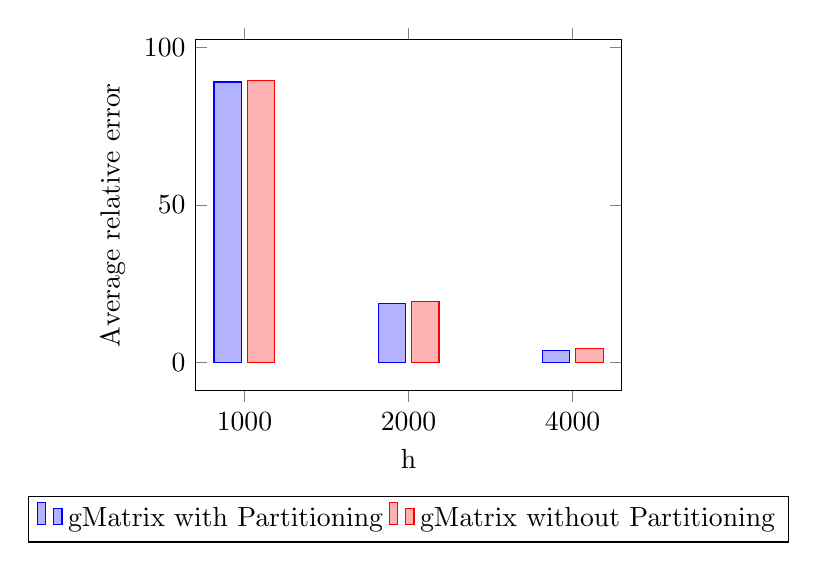
\begin{tikzpicture}
  \begin{axis}[
      ybar,
      enlargelimits=0.15,
      legend style={at={(0.5,-0.3)},anchor=north,legend columns=-1},
      ylabel={Average relative error},
      xlabel={h},
      width=7cm,
      symbolic x coords={1000,2000,4000},
      xtick=data
    ]
      \addplot 
	  coordinates {
        (1000,  88.956)
        (2000,  18.7822)
        (4000,  3.89071)
      };
      \addplot 
	  coordinates {
        (1000,  89.5238)
        (2000,  19.2599)
        (4000,  4.27863)
      };
      \legend{gMatrix with Partitioning,gMatrix without Partitioning}
  \end{axis}
\end{tikzpicture}
\caption{Average relative error on Twitter dataset considered over 1 million random edges} \label{fig:T21}
\end{figure}

\begin{figure}[!htbp]
\centering
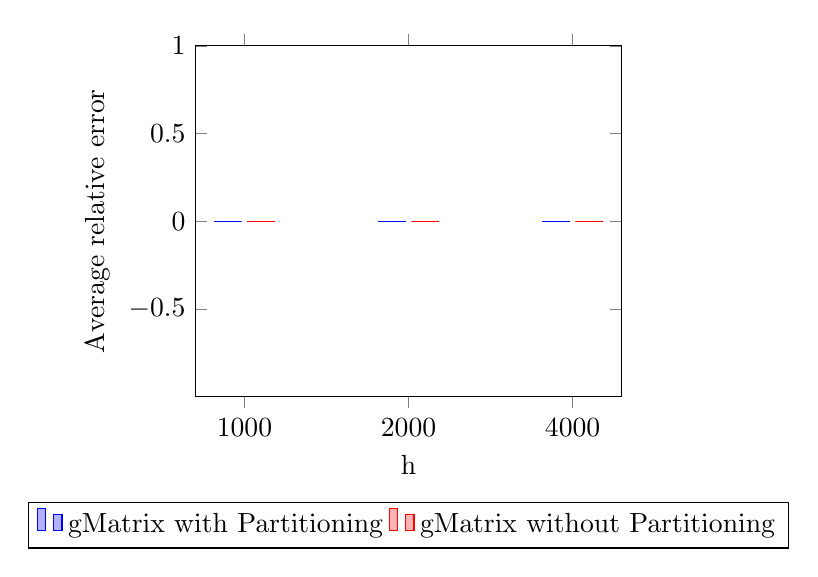
\begin{tikzpicture}
  \begin{axis}[
      ybar,
      enlargelimits=0.15,
      legend style={at={(0.5,-0.3)},anchor=north,legend columns=-1},
      ylabel={Average relative error},
      xlabel={h},
      width=7cm,
      symbolic x coords={1000,2000,4000},
      xtick=data
    ]
      \addplot 
	  coordinates {
        (1000,  0)
        (2000,  0)
        (4000,  0)
      };
      \addplot 
	  coordinates {
        (1000,  0)
        (2000,  0)
        (4000,  0)
      };
      \legend{gMatrix with Partitioning, gMatrix without Partitioning}
  \end{axis}
\end{tikzpicture}
\caption{Average relative error on Twitter dataset considered over top-500 highest frequency edges} \label{fig:T22}
\end{figure}

% Effective queries

\begin{figure}[!htbp]
\centering
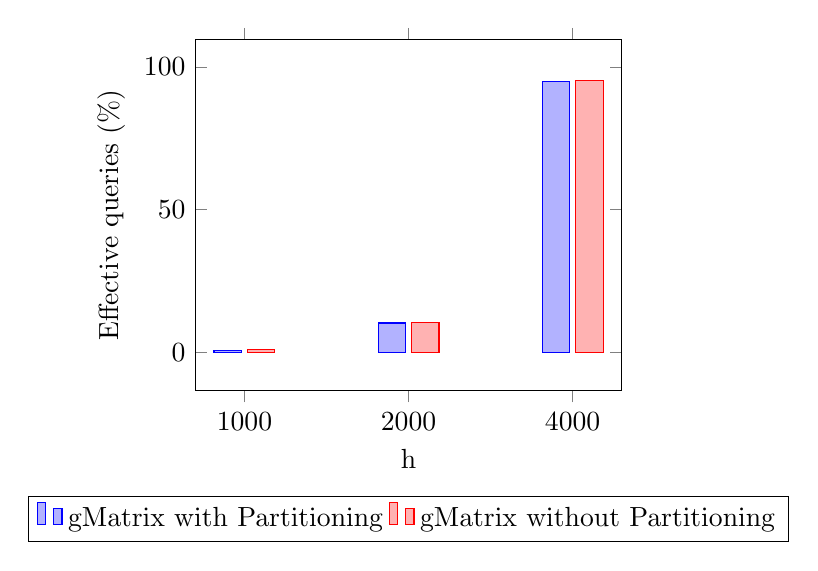
\begin{tikzpicture}
  \begin{axis}[
      ybar,
      enlargelimits=0.15,
      legend style={at={(0.5,-0.3)},anchor=north,legend columns=-1},
      ylabel={Effective queries (\%)},
      xlabel={h},
      width=7cm,
      symbolic x coords={1000,2000,4000},
      xtick=data
    ]
      \addplot 
	  coordinates {
        (1000,  0.6977)
        (2000,  10.214)
        (4000,  94.9675)
      };
      \addplot 
	  coordinates {
        (1000,  0.8046)
        (2000,  10.4912)
        (4000,  95.3025)
      };
      \legend{gMatrix with Partitioning,gMatrix without Partitioning}
  \end{axis}
\end{tikzpicture}
\caption{Effective queries percentage on Twitter dataset considered over 1 million random edges} \label{fig:T31}
\end{figure}

\begin{figure}[!htbp]
\centering
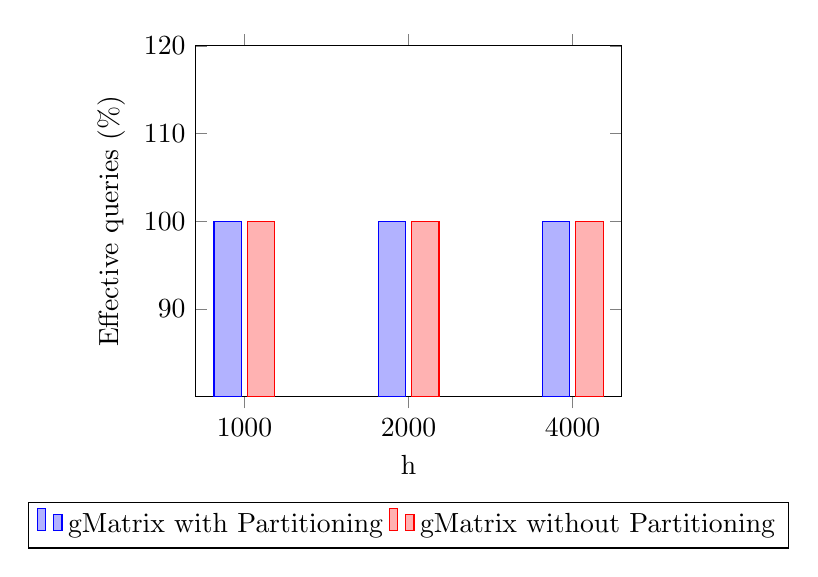
\begin{tikzpicture}
  \begin{axis}[
      ybar,
      enlargelimits=0.15,
      legend style={at={(0.5,-0.3)},anchor=north,legend columns=-1},
      ylabel={Effective queries (\%)},
      xlabel={h},
      width=7cm,
      symbolic x coords={1000,2000,4000},
      xtick=data
    ]
      \addplot 
	  coordinates {
        (1000,  100)
        (2000,  100)
        (4000,  100)
      };
      \addplot 
	  coordinates {
        (1000,  100)
        (2000,  100)
        (4000,  100)
      };
      \legend{gMatrix with Partitioning, gMatrix without Partitioning}
  \end{axis}
\end{tikzpicture}
\caption{Effective queries percentage on Twitter dataset considered over top-500 highest frequency edges} \label{fig:T32}
\end{figure}




%IP Trace
%Observed error
\begin{figure}[!htbp]
\centering
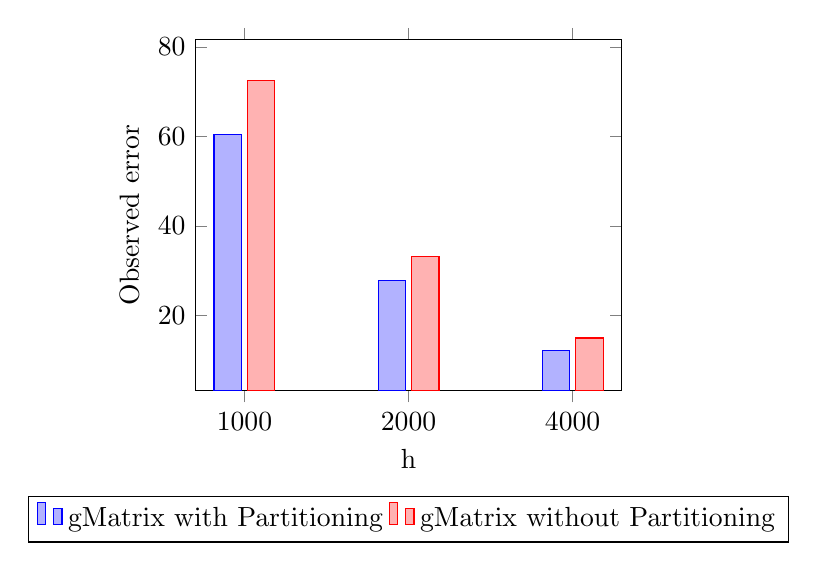
\begin{tikzpicture}
  \begin{axis}[
      ybar,
      enlargelimits=0.15,
      legend style={at={(0.5,-0.3)},anchor=north,legend columns=-1},
      ylabel={Observed error},
      xlabel={h},
      width=7cm,
      symbolic x coords={1000,2000,4000},
      xtick=data
    ]
      \addplot 
	  coordinates {
        (1000,  60.3821)
        (2000,  27.8266)
        (4000,  12.2106)
      };
      \addplot 
	  coordinates {
        (1000,  72.5277)
        (2000,  33.2313)
        (4000,  14.9191)
      };
      \legend{gMatrix with Partitioning,gMatrix without Partitioning}
  \end{axis}
\end{tikzpicture}
\caption{Observed error of IP-Trace dataset considered over 1 million random edges} \label{fig:I11}
\end{figure}

\begin{figure}[!htbp]
\centering
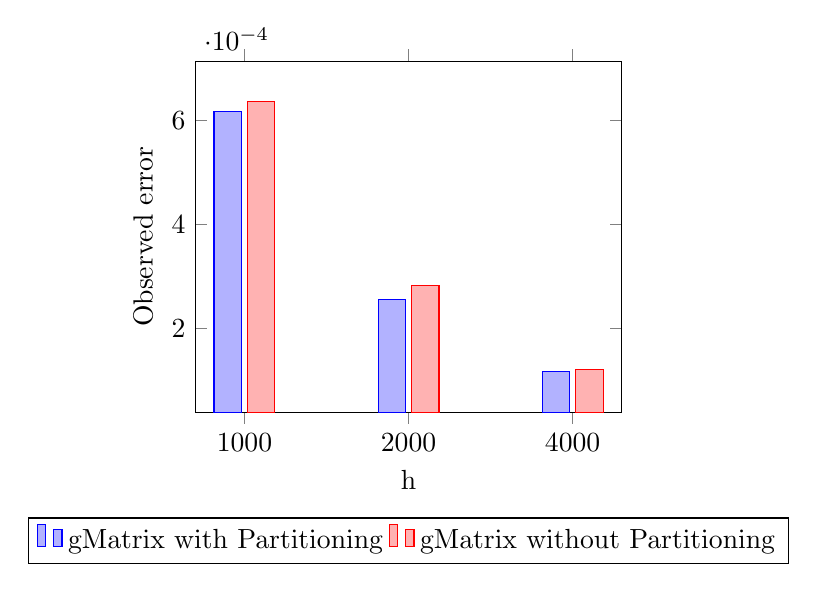
\begin{tikzpicture}
  \begin{axis}[
      ybar,
      enlargelimits=0.15,
      legend style={at={(0.5,-0.3)},anchor=north,legend columns=-1},
      ylabel={Observed error},
      xlabel={h},
      width=7cm,
      symbolic x coords={1000,2000,4000},
      xtick=data
    ]
      \addplot 
	  coordinates {
        (1000,  0.000616909)
        (2000,  0.000255977)
        (4000,  0.000116424)
      };
      \addplot 
	  coordinates {
        (1000,  0.000635283)
        (2000,  0.000282608)
        (4000,  0.000120565)
      };
      \legend{gMatrix with Partitioning, gMatrix without Partitioning}
  \end{axis}
\end{tikzpicture}
\caption{Observed error of IP-Trace dataset considered over top-500 highest frequency edges} \label{fig:I12}
\end{figure}

% Average relative error

\begin{figure}[!htbp]
\centering
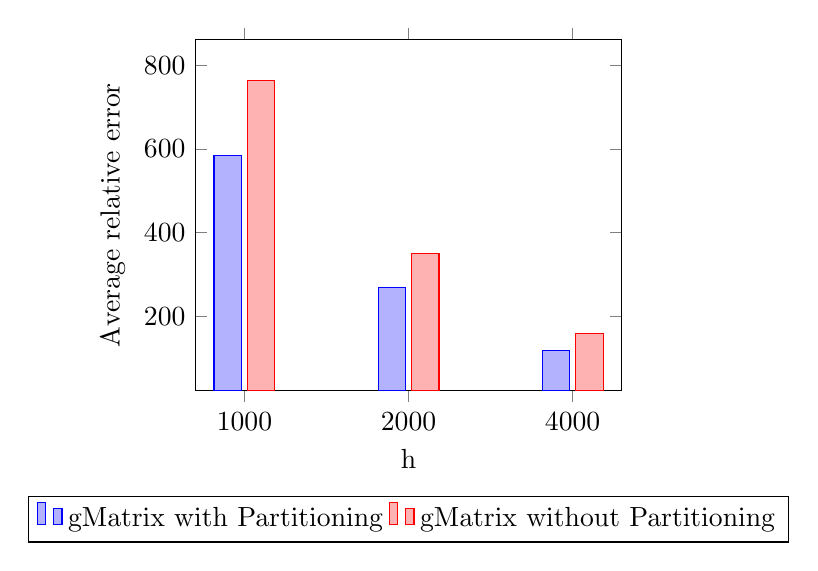
\begin{tikzpicture}
  \begin{axis}[
      ybar,
      enlargelimits=0.15,
      legend style={at={(0.5,-0.3)},anchor=north,legend columns=-1},
      ylabel={Average relative error},
      xlabel={h},
      width=7cm,
      symbolic x coords={1000,2000,4000},
      xtick=data
    ]
      \addplot 
	  coordinates {
        (1000,  583.576)
        (2000,  268.387)
        (4000,  118.987)
      };
      \addplot 
	  coordinates {
        (1000,  764.424)
        (2000,  350.601)
        (4000,  157.765)
      };
      \legend{gMatrix with Partitioning,gMatrix without Partitioning}
  \end{axis}
\end{tikzpicture}
\caption{Average relative error on IP-Trace dataset considered over 1 million random edges} \label{fig:I21}
\end{figure}

\begin{figure}[!htbp]
\centering
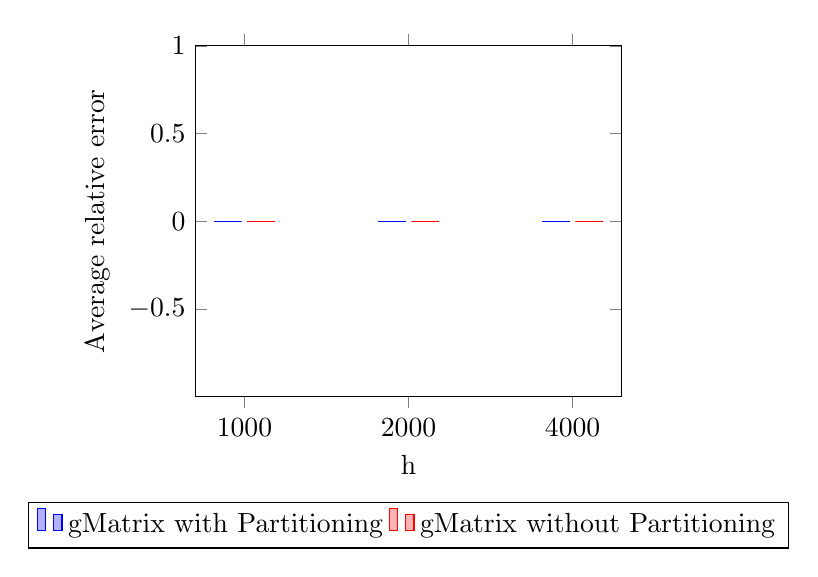
\begin{tikzpicture}
  \begin{axis}[
      ybar,
      enlargelimits=0.15,
      legend style={at={(0.5,-0.3)},anchor=north,legend columns=-1},
      ylabel={Average relative error},
      xlabel={h},
      width=7cm,
      symbolic x coords={1000,2000,4000},
      xtick=data
    ]
      \addplot 
	  coordinates {
        (1000,  0)
        (2000,  0)
        (4000,  0)
      };
      \addplot 
	  coordinates {
        (1000,  0)
        (2000,  0)
        (4000,  0)
      };
      \legend{gMatrix with Partitioning, gMatrix without Partitioning}
  \end{axis}
\end{tikzpicture}
\caption{Average relative error on IP-Trace dataset considered over top-500 highest frequency edges} \label{fig:I22}
\end{figure}

% Effective queries

\begin{figure}[!htbp]
\centering
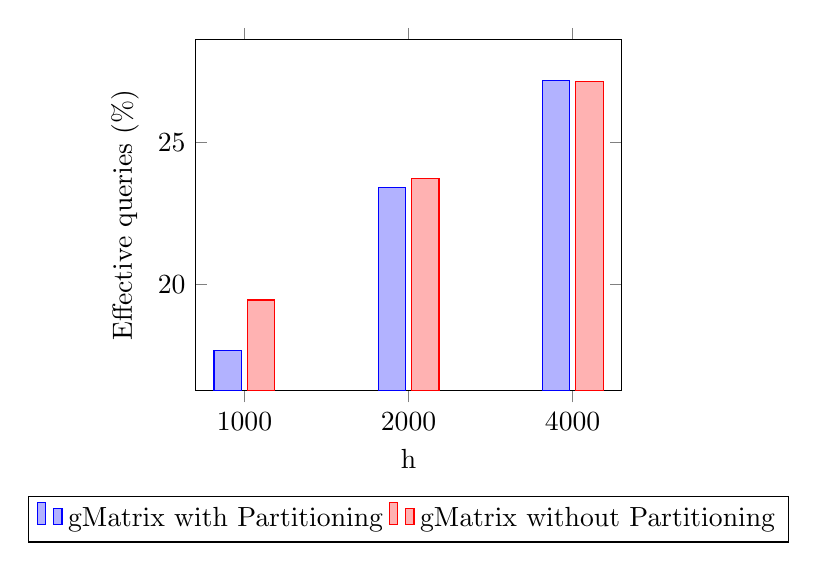
\begin{tikzpicture}
  \begin{axis}[
      ybar,
      enlargelimits=0.15,
      legend style={at={(0.5,-0.3)},anchor=north,legend columns=-1},
      ylabel={Effective queries (\%)},
      xlabel={h},
      width=7cm,
      symbolic x coords={1000,2000,4000},
      xtick=data
    ]
      \addplot 
	  coordinates {
        (1000,  17.6949)
        (2000,  23.426)
        (4000,  27.1898)
      };
      \addplot 
	  coordinates {
        (1000,  19.4597)
        (2000,  23.7307)
        (4000,  27.16)
      };
      \legend{gMatrix with Partitioning,gMatrix without Partitioning}
  \end{axis}
\end{tikzpicture}
\caption{Effective queries percentage on IP-Trace dataset considered over 1 million random edges} \label{fig:I31}
\end{figure}

\begin{figure}[!htbp]
\centering
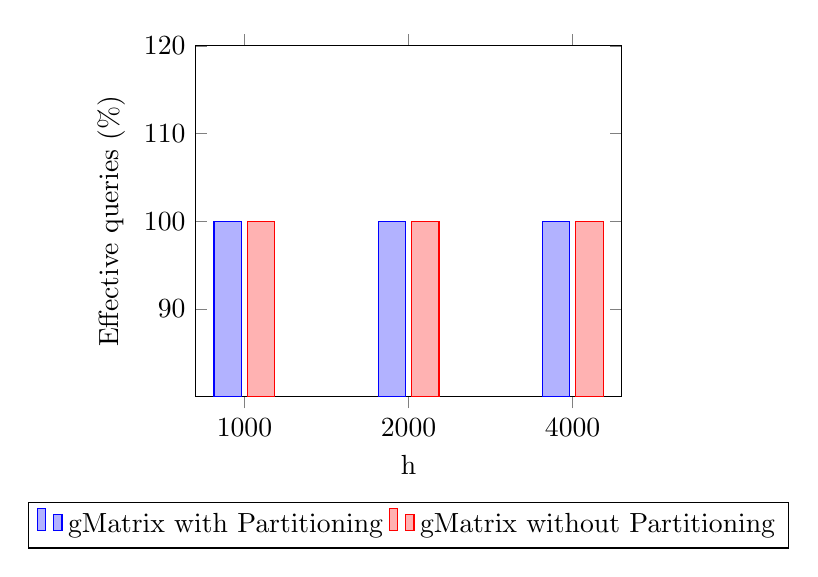
\begin{tikzpicture}
  \begin{axis}[
      ybar,
      enlargelimits=0.15,
      legend style={at={(0.5,-0.3)},anchor=north,legend columns=-1},
      ylabel={Effective queries (\%)},
      xlabel={h},
      width=7cm,
      symbolic x coords={1000,2000,4000},
      xtick=data
    ]
      \addplot 
	  coordinates {
        (1000,  100)
        (2000,  100)
        (4000,  100)
      };
      \addplot 
	  coordinates {
        (1000,  100)
        (2000,  100)
        (4000,  100)
      };
      \legend{gMatrix with Partitioning, gMatrix without Partitioning}
  \end{axis}
\end{tikzpicture}
\caption{Effective queries percentage on IP-Trace dataset considered over top-500 highest frequency edges} \label{fig:I32}
\end{figure}

% Heavy hitter

\clearpage
\subsection{Heavy Hitter Edge Estimation}

Figures \ref{fig:EE1} and \ref{fig:EE2} show that after partitioning, the sketch is more sensitive to low frequency thresholds as the false positive rates are much higher at frequency threshold of 0.01\% of the total stream frequency. However, it performs as good at frequency threshold percentages of 0.1\% and 1\%, with no false positives produced at all.

\begin{figure}[!htbp]
\centering
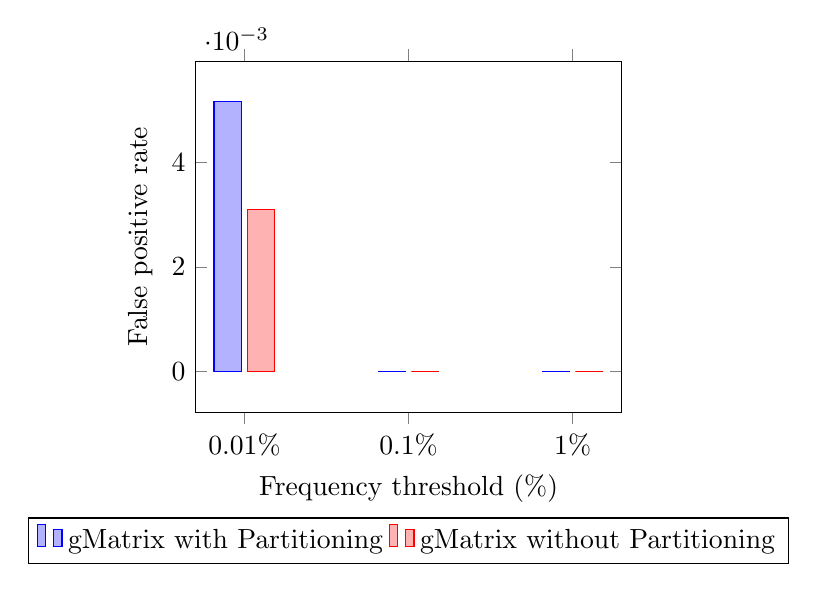
\begin{tikzpicture}
  \begin{axis}[
      ybar,
      enlargelimits=0.15,
      legend style={at={(0.5,-0.3)},anchor=north,legend columns=-1},
      ylabel={False positive rate},
      xlabel={Frequency threshold (\%)},
      width=7cm,
      symbolic x coords={0.01\%,0.1\%,1\%},
      xtick=data
    ]
      \addplot 
	  coordinates {
        (0.01\%,0.00515996)
        (0.1\%, 0)
        (1\%,   0)
      };
      \addplot 
	  coordinates {
        (0.01\%,  0.00309598)
        (0.1\%,   0)
        (1\%,     0)
      };
      \legend{gMatrix with Partitioning, gMatrix without Partitioning}
  \end{axis}
\end{tikzpicture}
\caption{False positive rate of heavy hitter edge estimation on IP-Trace dataset with respect to varying frequency threshold percentages of the total stream frequency} \label{fig:EE1}
\end{figure}

\begin{figure}[!htbp]
\centering
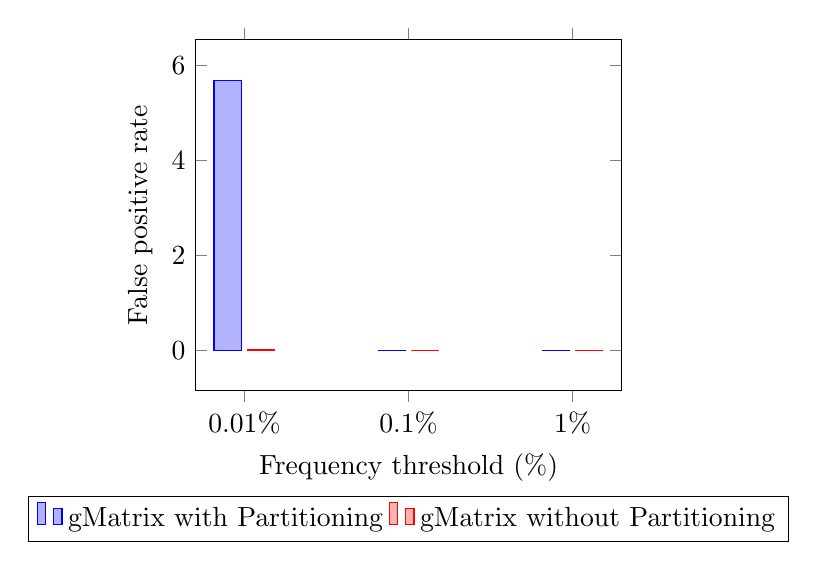
\begin{tikzpicture}
  \begin{axis}[
      ybar,
      enlargelimits=0.15,
      legend style={at={(0.5,-0.3)},anchor=north,legend columns=-1},
      ylabel={False positive rate},
      xlabel={Frequency threshold (\%)},
      width=7cm,
      symbolic x coords={0.01\%,0.1\%,1\%},
      xtick=data
    ]
      \addplot 
	  coordinates {
        (0.01\%,5.691796)
        (0.1\%, 0)
        (1\%,   0)
      };
      \addplot 
	  coordinates {
        (0.01\%,  0.015521)
        (0.1\%,   0)
        (1\%,     0)
      };
      \legend{gMatrix with Partitioning, gMatrix without Partitioning}
  \end{axis}
\end{tikzpicture}
\caption{False positive rate of heavy hitter edge estimation on Friendster dataset with respect to varying frequency threshold percentages of the total stream frequency} \label{fig:EE2}
\end{figure}

%Node Aggregate
\clearpage
\subsection{Node Aggregate-Frequency Estimation}

On the Twitter and IP-Trace dataset, the observed error of source-node aggregate-frequency estimations is lower after partitioning as seen on figure \ref{fig:agg3} and figure \ref{fig:agg5}. However, on the Friendster dataset, figure \ref{fig:agg1} shows that it is higher after partitioning, which is unexpected. According to Theorem \ref{thm:agg1}, an ideal partitioning scheme improves accuracy guarantee, although reduces the probability of the guarantee. We speculate that the higher observed error on the Friendster dataset is due to the high-skewness of the dataset, which makes the partitioning scheme less effective.

Figures \ref{fig:agg2}, \ref{fig:agg4} and \ref{fig:agg6} show the observed error is higher after partitioning in destination-node aggregate-frequency estimations, which is expected since Theorem \ref{thm:agg2} shows that partitioning does not improve the accuracy guarantee itself and only worsens the probability of the guarantee.

\begin{figure}[!htbp]
\centering
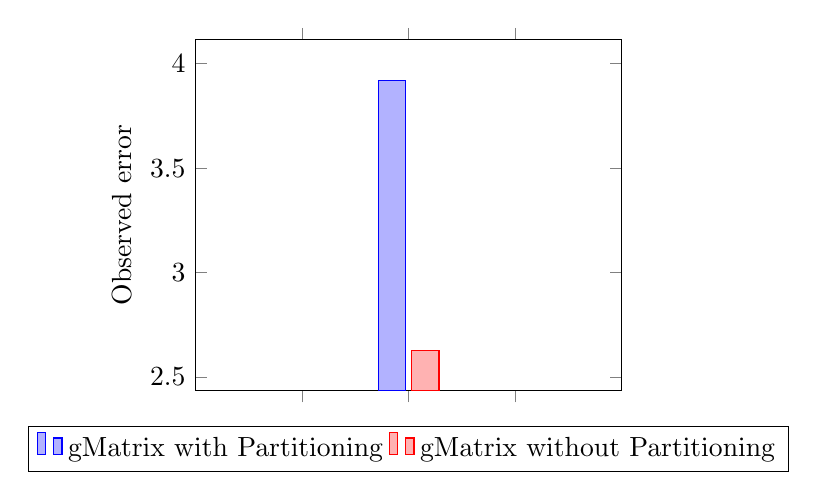
\begin{tikzpicture}
  \begin{axis}[
      ybar,
      enlargelimits=0.15,
      legend style={at={(0.5,-0.1)},anchor=north,legend columns=-1},
      ylabel={Observed error},
      width=7cm,
      xticklabels={,,}
    ]
      \addplot 
	  coordinates {
        (0, 3.920681)
      };
      \addplot 
	  coordinates {
        (0, 2.628615)
      };
      \legend{gMatrix with Partitioning,gMatrix without Partitioning}
  \end{axis}
\end{tikzpicture}
\caption{Observed error of source-node aggregate-frequency queries on top-500 node aggregate-frequencies of the Friendster dataset} \label{fig:agg1}
\end{figure}

\begin{figure}[!htbp]
\centering
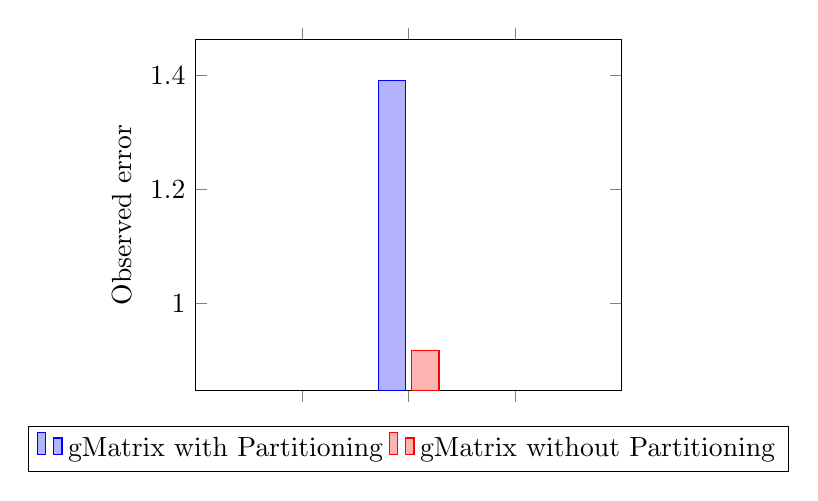
\begin{tikzpicture}
  \begin{axis}[
      ybar,
      enlargelimits=0.15,
      legend style={at={(0.5,-0.1)},anchor=north,legend columns=-1},
      ylabel={Observed error},
      width=7cm,
      xticklabels={,,}
    ]
      \addplot 
	  coordinates {
        (0, 1.391630)
      };
      \addplot 
	  coordinates {
        (0, 0.918388)
      };
      \legend{gMatrix with Partitioning,gMatrix without Partitioning}
  \end{axis}
\end{tikzpicture}
\caption{Observed error of destination-node aggregate-frequency queries on top-500 node aggregate-frequencies of the Friendster dataset} \label{fig:agg2}
\end{figure}

\begin{figure}[!htbp]
\centering
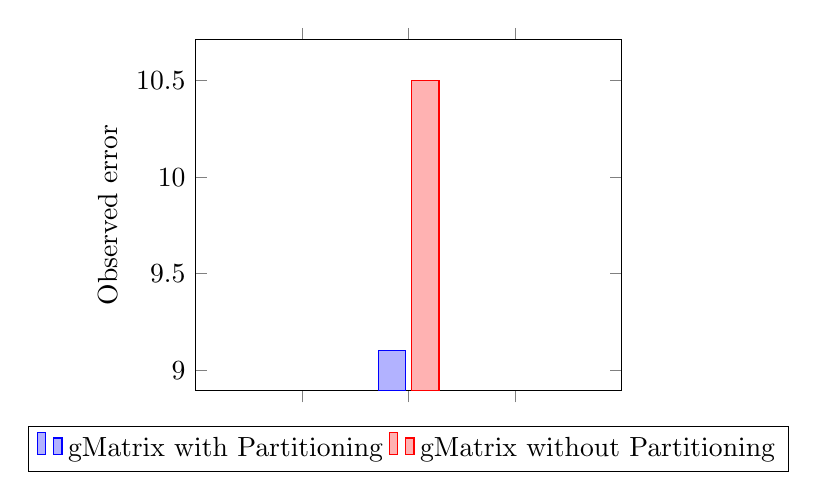
\begin{tikzpicture}
  \begin{axis}[
      ybar,
      enlargelimits=0.15,
      legend style={at={(0.5,-0.1)},anchor=north,legend columns=-1},
      ylabel={Observed error},
      width=7cm,
      xticklabels={,,}
    ]
      \addplot 
	  coordinates {
        (0, 9.104631)
      };
      \addplot 
	  coordinates {
        (0, 10.501604)
      };
      \legend{gMatrix with Partitioning,gMatrix without Partitioning}
  \end{axis}
\end{tikzpicture}
\caption{Observed error of source-node aggregate-frequency queries on top-500 node aggregate-frequencies of the Twitter dataset} \label{fig:agg3}
\end{figure}

\begin{figure}[!htbp]
\centering
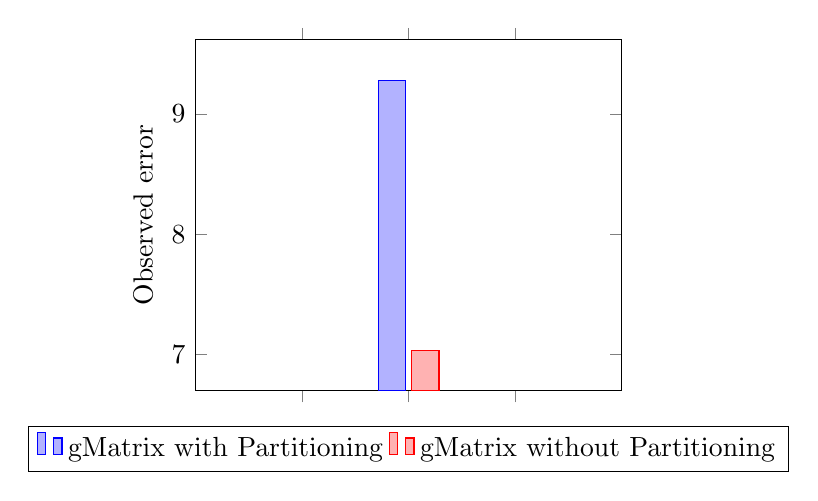
\begin{tikzpicture}
  \begin{axis}[
      ybar,
      enlargelimits=0.15,
      legend style={at={(0.5,-0.1)},anchor=north,legend columns=-1},
      ylabel={Observed error},
      width=7cm,
      xticklabels={,,}
    ]
      \addplot 
	  coordinates {
        (0, 9.279370)
      };
      \addplot 
	  coordinates {
        (0, 7.038425)
      };
      \legend{gMatrix with Partitioning,gMatrix without Partitioning}
  \end{axis}
\end{tikzpicture}
\caption{Observed error of destination-node aggregate-frequency queries on top-500 node aggregate-frequencies of the Twitter dataset} \label{fig:agg4}
\end{figure}


\begin{figure}[!htbp]
\centering
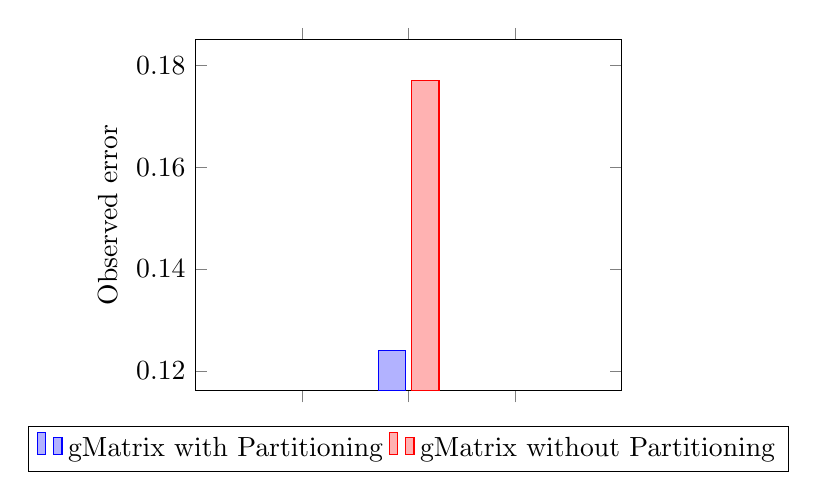
\begin{tikzpicture}
  \begin{axis}[
      ybar,
      enlargelimits=0.15,
      legend style={at={(0.5,-0.1)},anchor=north,legend columns=-1},
      ylabel={Observed error},
      width=7cm,
      xticklabels={,,}
    ]
      \addplot 
	  coordinates {
        (0, 0.124063)
      };
      \addplot 
	  coordinates {
        (0, 0.177073)
      };
      \legend{gMatrix with Partitioning,gMatrix without Partitioning}
  \end{axis}
\end{tikzpicture}
\caption{Observed error of source-node aggregate-frequency queries on top-500 node aggregate-frequencies of the IP-Trace dataset} \label{fig:agg5}
\end{figure}

\begin{figure}[!htbp]
\centering
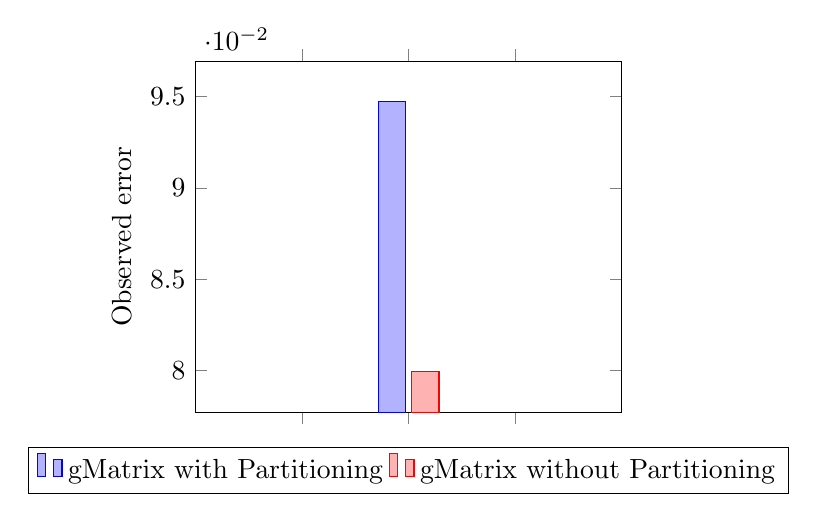
\begin{tikzpicture}
  \begin{axis}[
      ybar,
      enlargelimits=0.15,
      legend style={at={(0.5,-0.1)},anchor=north,legend columns=-1},
      ylabel={Observed error},
      width=7cm,
      xticklabels={,,}
    ]
      \addplot 
	  coordinates {
        (0, 0.094721)
      };
      \addplot 
	  coordinates {
        (0, 0.079930)
      };
      \legend{gMatrix with Partitioning,gMatrix without Partitioning}
  \end{axis}
\end{tikzpicture}
\caption{Observed error of destination-node aggregate-frequency queries on top-500 node aggregate-frequencies of the IP-Trace dataset} \label{fig:agg6}
\end{figure}

%!TEX root = ../thesis.tex
%*******************************************************************************
%****************************** Third Chapter **********************************
%*******************************************************************************
\chapter{Conclusions}

% **************************** Define Graphics Path **************************
\ifpdf
\graphicspath{{Chapter4/Figs/Raster/}{Chapter4/Figs/PDF/}{Chapter4/Figs/}}
\else
\graphicspath{{Chapter4/Figs/Vector/}{Chapter4/Figs/}}
\fi

\section{Conclusion}

To summarize all contributions made so far, we have proposed optimizations to the partitioning method, analyzes how the method impacts how the gMatrix sketch answers various query types and how the performance and accuracy guarantees change, and conducted experiments on some datasets.

The results show that the gSketch partitioning method generally improves gMatrix accuracy on query types such as edge frequency and source-node aggregate frequency estimations. In addition, such queries are performed with the same time complexity too.

However, the gSketch partitioning method causes gMatrix to be less accurate and to be slower on some query types such as the destination-node aggregate frequency estimation and the heavy-hitter edge queries.

Finally, we note that whether the partitioning method is beneficial for use depends on the intended use-case.

\section{Possible Improvements}

Experiments on how the partitioning method affects gMatrix on other query types supported by the gMatrix are yet to be conducted. In addition, experiments on the effects of varying the partitioning parameters on the gMatrix are yet to be conducted too. Finally, experiments on other datasets may produce new insights.

%\include{Chapter5/chapter5}
%\include{Chapter6/chapter6}
%\include{Chapter7/chapter7}



% ********************************** Back Matter *******************************
% Backmatter should be commented out, if you are using appendices after References
%\backmatter

% ********************************** Bibliography ******************************
\begin{spacing}{0.9}

% To use the conventional natbib style referencing
% Bibliography style previews: http://nodonn.tipido.net/bibstyle.php
% Reference styles: http://sites.stat.psu.edu/~surajit/present/bib.htm

\bibliographystyle{apalike}
%\bibliographystyle{unsrt} % Use for unsorted references  
%\bibliographystyle{plainnat} % use this to have URLs listed in References
\cleardoublepage
\bibliography{References/references} % Path to your References.bib file


% If you would like to use BibLaTeX for your references, pass `custombib' as
% an option in the document class. The location of 'reference.bib' should be
% specified in the preamble.tex file in the custombib section.
% Comment out the lines related to natbib above and uncomment the following line.

%\printbibliography[heading=bibintoc, title={References}]


\end{spacing}

% ********************************** Appendices ********************************

%\begin{appendices} % Using appendices environment for more functunality

%%!TEX root = ../thesis.tex
% ******************************* Thesis Appendix A ****************************
\chapter{How to install \LaTeX} 

\section*{Windows OS}

\subsection*{TeXLive package - full version}
\begin{enumerate}
\item	Download the TeXLive ISO (2.2GB) from\\
\href{https://www.tug.org/texlive/}{https://www.tug.org/texlive/}
\item	Download WinCDEmu (if you don't have a virtual drive) from \\
\href{http://wincdemu.sysprogs.org/download/}
{http://wincdemu.sysprogs.org/download/}
\item	To install Windows CD Emulator follow the instructions at\\
\href{http://wincdemu.sysprogs.org/tutorials/install/}
{http://wincdemu.sysprogs.org/tutorials/install/}
\item	Right click the iso and mount it using the WinCDEmu as shown in \\
\href{http://wincdemu.sysprogs.org/tutorials/mount/}{
http://wincdemu.sysprogs.org/tutorials/mount/}
\item	Open your virtual drive and run setup.pl
\end{enumerate}

or

\subsection*{Basic MikTeX - \TeX~ distribution}
\begin{enumerate}
\item	Download Basic-MiK\TeX (32bit or 64bit) from\\
\href{http://miktex.org/download}{http://miktex.org/download}
\item	Run the installer 
\item	To add a new package go to Start >> All Programs >> MikTex >> Maintenance (Admin) and choose Package Manager
\item	Select or search for packages to install
\end{enumerate}

\subsection*{TexStudio - \TeX~ editor}
\begin{enumerate}
\item	Download TexStudio from\\
\href{http://texstudio.sourceforge.net/\#downloads}
{http://texstudio.sourceforge.net/\#downloads} 
\item	Run the installer
\end{enumerate}

\section*{Mac OS X}
\subsection*{MacTeX - \TeX~ distribution}
\begin{enumerate}
\item	Download the file from\\
\href{https://www.tug.org/mactex/}{https://www.tug.org/mactex/}
\item	Extract and double click to run the installer. It does the entire configuration, sit back and relax.
\end{enumerate}

\subsection*{TexStudio - \TeX~ editor}
\begin{enumerate}
\item	Download TexStudio from\\
\href{http://texstudio.sourceforge.net/\#downloads}
{http://texstudio.sourceforge.net/\#downloads} 
\item	Extract and Start
\end{enumerate}


\section*{Unix/Linux}
\subsection*{TeXLive - \TeX~ distribution}
\subsubsection*{Getting the distribution:}
\begin{enumerate}
\item	TexLive can be downloaded from\\
\href{http://www.tug.org/texlive/acquire-netinstall.html}
{http://www.tug.org/texlive/acquire-netinstall.html}.
\item	TexLive is provided by most operating system you can use (rpm,apt-get or yum) to get TexLive distributions
\end{enumerate}

\subsubsection*{Installation}
\begin{enumerate}
\item	Mount the ISO file in the mnt directory
\begin{verbatim}
mount -t iso9660 -o ro,loop,noauto /your/texlive####.iso /mnt
\end{verbatim}

\item	Install wget on your OS (use rpm, apt-get or yum install)
\item	Run the installer script install-tl.
\begin{verbatim}
	cd /your/download/directory
	./install-tl
\end{verbatim}
\item	Enter command `i' for installation

\item	Post-Installation configuration:\\
\href{http://www.tug.org/texlive/doc/texlive-en/texlive-en.html\#x1-320003.4.1}
{http://www.tug.org/texlive/doc/texlive-en/texlive-en.html\#x1-320003.4.1} 
\item	Set the path for the directory of TexLive binaries in your .bashrc file
\end{enumerate}

\subsubsection*{For 32bit OS}
For Bourne-compatible shells such as bash, and using Intel x86 GNU/Linux and a default directory setup as an example, the file to edit might be \begin{verbatim}
edit $~/.bashrc file and add following lines
PATH=/usr/local/texlive/2011/bin/i386-linux:$PATH; 
export PATH 
MANPATH=/usr/local/texlive/2011/texmf/doc/man:$MANPATH;
export MANPATH 
INFOPATH=/usr/local/texlive/2011/texmf/doc/info:$INFOPATH;
export INFOPATH
\end{verbatim}
\subsubsection*{For 64bit OS}
\begin{verbatim}
edit $~/.bashrc file and add following lines
PATH=/usr/local/texlive/2011/bin/x86_64-linux:$PATH;
export PATH 
MANPATH=/usr/local/texlive/2011/texmf/doc/man:$MANPATH;
export MANPATH 
INFOPATH=/usr/local/texlive/2011/texmf/doc/info:$INFOPATH;
export INFOPATH

\end{verbatim}



%\subsection{Installing directly using Linux packages} 
\subsubsection*{Fedora/RedHat/CentOS:}
\begin{verbatim} 
sudo yum install texlive 
sudo yum install psutils 
\end{verbatim}


\subsubsection*{SUSE:}
\begin{verbatim}
sudo zypper install texlive
\end{verbatim}


\subsubsection*{Debian/Ubuntu:}
\begin{verbatim} 
sudo apt-get install texlive texlive-latex-extra 
sudo apt-get install psutils
\end{verbatim}

%%!TEX root = ../thesis.tex
% ******************************* Thesis Appendix B ********************************

\chapter{Installing the CUED class file}

\LaTeX.cls files can be accessed system-wide when they are placed in the
<texmf>/tex/latex directory, where <texmf> is the root directory of the user’s \TeX installation. On systems that have a local texmf tree (<texmflocal>), which
may be named ``texmf-local'' or ``localtexmf'', it may be advisable to install packages in <texmflocal>, rather than <texmf> as the contents of the former, unlike that of the latter, are preserved after the \LaTeX system is reinstalled and/or upgraded.

It is recommended that the user create a subdirectory <texmf>/tex/latex/CUED for all CUED related \LaTeX class and package files. On some \LaTeX systems, the directory look-up tables will need to be refreshed after making additions or deletions to the system files. For \TeX Live systems this is accomplished via executing ``texhash'' as root. MIK\TeX users can run ``initexmf -u'' to accomplish the same thing.

Users not willing or able to install the files system-wide can install them in their personal directories, but will then have to provide the path (full or relative) in addition to the filename when referring to them in \LaTeX.

%\end{appendices}

% *************************************** Index ********************************
\printthesisindex % If index is present

\end{document}
